\documentclass{uofsthesis-cs}

\usepackage{graphicx, amsmath, caption, verbatim, subfig, booktabs, multirow, bm}

% Documentation for the uofsthesis-cs class is given in uofsthesis-cs.dvi
% 
% It is recommended that you read the CGSR thesis preparation
% guidelines before proceeding.
% They can be found at http://www.usask.ca/cgsr/thesis/index.htm

%%%%%%%%%%%%%%%%%%%%%%%%%%%%%%%%%%%%%%%%%%%%%%%%%%%%%%%%%%%%%%%%%%%%%%%%%%%%%%
% FRONTMATTER - In this section, specify information to be used to
% typeset the thesis frontmatter.
%%%%%%%%%%%%%%%%%%%%%%%%%%%%%%%%%%%%%%%%%%%%%%%%%%%%%%%%%%%%%%%%%%%%%%%%%%%%%%

% THESIS TITLE
% Specify the title. Set the capitalization how you want it.
\title{Home Advantage in North American Professional Sports Before and During COVID-19: A Bayesian Perspective}
% AUTHOR'S NAME
% Your name goes here.
\author{Nicholas Higgs}

% DEGREE SOUGHT.  
% Use \MSc or \PhD here
\degree{\MSc}

% THESIS DEFENCE DATE
% Should be month year, e.g. July 2004
\defencedate{Month Year}


% NAME OF ACADEMIC UNIT
%
% The following two commands allow you to specify the academic unit you belong to.
% This will appear on the title page as
% ``<academic unit> of <department>''.
% So if you are in the division of biomedical engineering you would need to do:
% \department{Biomedical Engineering}
% \academicunit{Division}
%
% The default is ``Department of Computer Science'' if these commands
% are not given.
%
% If you are in a discipline other than Computer Science, uncomment the following line and
% specify your discipline/department.  Default is 'Computer Science'.
% \department{If not Computer Science, put the name of your department here}

% If you are not in a department, but say, a division, uncomment the following line.
% \academicunit{Put the type of academic unit you belong to here, e.g. Division, College}


% PERMISSION TO USE ADDRESS
%
% If you are not in Comptuer Science you will want to change the
% address on the Permission to Use page.  This is done using the
% \ptuaddress{}.  Example:
%
% \ptuaddress{Head of the Department of Computer Science\\
% 176 Thorvaldson Building\\
% 110 Science Place\\
% University of Saskatchewan\\
% Saskatoon, Saskatchewan\\
% Canada\\
% S7N 5C9
% }

% ABSTRACT
\abstract{
This is the abstract of my thesis.  
}

% THESIS ACKNOWLEDGEMENTS -- This can be free-form.
\acknowledgements{
Acknowledgements go here.  Typically you would at least thank your supervisor.
}

% THESIS DEDICATION -- Also free-form.  If you don't want a dedication, comment out the following
% line.
\dedication{This is the thesis dedication (optional)}

% LIST OF ABBREVIATIONS - Sample  
% If you don't want a list of abbreviations, comment the following 4 lines.
\loa{
\abbrev{SCUBA}{Self Contained Underwater Breathing Apparatus\hfill}
\abbrev{LOF}{List of Figures}
\abbrev{LOT}{List of Tables}
}

%%%%%%%%%%%%%%%%%%%%%%%%%%%%%%%%%%%%%%%%%%%%%%%%%%%%%%%%%%%%%%%%
% END OF FRONTMATTER SECTION
%%%%%%%%%%%%%%%%%%%%%%%%%%%%%%%%%%%%%%%%%%%%%%%%%%%%%%%%%%%%%%%%

\begin{document}
% Typeset the title page
\maketitle
\tracingall1

% Typeset the frontmatter.  
\frontmatter

%%%%%%%%%%%%%%%%%%%%%%%%%%%%%%%%%%%%%%%%%%%%%%%%%%%%%%%%%%%%%%%%
% FIRST CHAPTER OF THESIS BEGINS HERE
%%%%%%%%%%%%%%%%%%%%%%%%%%%%%%%%%%%%%%%%%%%%%%%%%%%%%%%%%%%%%%%%

\chapter{Introduction}

In professional sports, home teams tend to win more on average than visiting teams \cite{Schwartz1977} \cite{Courneya1992} \cite{Nevill1999}. This phenomenon has been widely studied across several fields including psychology \cite{Agnew1994} \cite{Unkelbach2010}, economics \cite{Forrest2005} \cite{Dohmen2016}, and statistics \cite{Buraimo2010} \cite{Lopez2018} among others \cite{Benz2020}. While home advantage is now a widely accepted phenomenon, the magnitude of the advantage and its cause are not as clearly understood or widely accepted as its existence. Part of the difficulty in analyzing the specifics of home advantage is due to the lack of controlled experiments, because nearly every professional game is played in one of the team's home stadium in their home city. While there have existed some show matches at neutral sites, their relative sample sizes are too small from which to draw any reasonable conclusions. For example, the National Football League only plays about 4-5 neutral site games out of a total 256 games each regular season.

The return to play of professional sports during the COVID-19 pandemic presents a unique opportunity to analyze teams playing in situations where home advantage may genuinely no longer apply. The leagues have restricted travel and fan attendance or even created a bubble where only one or two stadiums are used and only the players and necessary staff are present for the games. We consider this restricted return to play as a control group where travel, home stadium familiarity, and home crowd have been controlled (i.e. removed) for enough games to provide a reasonable sample to analyze. There has been considerable academic work analyzing the effect of COVID-19 restrictions on home advantage in European football \cite{Benz2020}. However, comparatively there has been a lack of work analyzing the effect in the North American professional sports leagues. In fact, to the authors knowledge there has only been one work focused on home advantage during COVID-19 across the big four North American professional leagues; and it only investigated the NBA \cite{McHill2020}. In this work, we aim to fill this gap by inferring the effect of and changes in home advantage prior to and during COVID-19 in the big four North American leagues: the National Hockey League (NHL), the National Basketball Association (NBA), Major League Baseball (MLB), and the National Football League (NFL).

Professional sports leagues adopted different restrictions in response to the COVID-19 pandemic. The NHL and NBA had the strongest restrictions where they both created a COVID-19 bubble where all games were played at the same consistent location with players quarantined together separate from their families and the outside world. While this proved to be extremely effective in terms of player safety \cite{nhl2020} \cite{usatoday2020} it seems likely that it was the most extreme in terms of its effect on players performance and psychology. In contrast, teams in the MLB and NFL still traveled to their opponents home stadiums. These leagues restricted fan attendance and media access, with some NFL stadiums allowing small amounts of fans to attend. Thus, all leagues lacked a potential home crowd effect, but only the NHL and NBA restrictions removed the additional factors of travel and home city familiarity. This is noteworthy because of the implications in relation to previous work investigating the causes of home advantage  \cite{Unkelbach2010} \cite{Buraimo2010} \cite{Courneya1992} \cite{Carron2005} \cite{McHill2020} \cite{Garicano2005} \cite{Moskowitz2012}. In McHill \& Chinoy \cite{McHill2020}, the authors argue that home advantage in the NBA's COVID-19 bubble arose from either circadian disruption or the general effect of travel. Our work builds upon such previous works by considering the NBA's COVID-19 bubble and its effects on home advantage while also comparing and contrasting to other similar COVID-19 bubbles in the NHL and different COVID-19 restrictions seen in the MLB and NFL.

\subsection{Contribution}

We adopt a Bayesian framework to develop a Negative Binomial regression model that adjusts for relative team strengths while inferring home advantage. We choose this approach for two main reasons. First, alternative methods that rely on correlations among raw statistics, such as home win percentage, fail to account for other factors such as relative team strengths. Our regression approach can infer changes in team performance while adjusting for quality of opponents. Second, the Bayesian framework gives more interpretable results and more flexibility in model building than classical regression methods. The Bayesian framework results in distributions for the estimates of each parameter in our model. This allows us to analyze these distributions directly to determine the probability a parameter is greater (less) than a certain value or that it exists in a specific interval, avoiding the confusion that often arises interpreting p-values and confidence intervals.

By examining the resulting home advantage parameter estimates of our model from before and during the COVID-19 pandemic, we can draw conclusions about the existence of the home advantage phenomenon and provide new evidence for its potential causes. We hypothesize that home advantage is a real phenomenon, thus we expect its parameter estimate to drop during the COVID-19 seasons relative to before the COVID-19 seasons. We are also interested in examining if any differences in relative changes in home advantage exist across the leagues as some leagues had different COVID-19 restrictions which could affect home advantage differently. We also show that point totals in North American professional sports are prone to overdispersion, thus, the Negative Binomial distribution allows for better model fit than the more common Poisson and Normal distributions used in regression analyses.

- the above is almost verbatim the paper. Since the thesis has an additional experiment I think I either need to add a paragraph to describe what is to come in each chapter, or I need to somehow embed the new/additional thesis work into the above.

The rest of the thesis is organized as follows. The background chapter provides an introduction to Bayesian statistics, multi-level modelling, fitting Bayesian models via Markov Chain Monte Carlo sampling, and evaluating models. The methods chapter describes in-depth the Bayesian multi-level regression that was developed to infer home advantage, and how the various data experiments for the mainc contributions of this work are set up. The results chapter presents and discusses the results of the experiments introduced in the methods chapter. The conclusion chapter contains a discussion of the results and their implications while summarizing the findings and contributions of the thesis.


% Since thesis chapters are very long and there are a lot of them, it is recommended
% that you put each chapter in a separate .tex file and \input each one of them
% in order.  For example:
%
% \input chap1.tex
% \input chap2.tex
% ...
%
% The \input command inserts contents of the specified file at the point of the command.

%%%%%%%%%%%%%%%%%%%%%%%%%%%%%%%%%%%%%%%%%%%%%%%%%%%%%%%%%%%%%%%
% SUBSEQUENT CHAPTERS (or \input's)  GO HERE
%%%%%%%%%%%%%%%%%%%%%%%%%%%%%%%%%%%%%%%%%%%%%%%%%%%%%%%%%%%%%%%

\chapter{Background}
\section{Home Advantage}
\subsection{Related Work}

The initially most well known and cited work on home advantage in sports was done in 1977 by Schwartz and Barsky \cite{Schwartz1977} who analyzed and found home advantage to exist in professional hockey, basketball, baseball and football. In \cite{Courneya1992} the authors accept home advantage as a real phenomena after reviewing the relevant literature and argue for a framework that focuses on game location, psychological states, behavioral states, and performance outcomes to try to understand the underlying causes of home advantage. Follow up work a decade later by Carron et al. \cite{Carron2005} reviewed the literature and concluded that home advantage was still present in both amateur and professional sports, in both individual and team sports, across genders, and across time. More recent works \cite{Pollard2005a} \cite{Gomez2011} confirm the continued existence of home advantage in the North American professional leagues we are considering in this study: the NHL, NBA, NFL, and MLB. In general, older studies on home advantage tend to use correlation methods of aggregated full season statistics (e.g. combining all teams home wins into one home win percentage to see if it is above 50\%), whereas more recent studies more often build statistical regression models from game level data that adjust for additional factors, such as relative team strengths, and try to infer the effect of the home advantage parameter on the regression model.

There have been several studies analyzing home advantage in the context of COVID-19 adjusted seasons; however, nearly all of them have focused exclusively on European Soccer leagues. In \cite{Benz2020} thirteen such works are summarized, of which only two used correlation methods and the other eleven made use of regression analysis to infer the change in home advantage. Benz and Lopez themselves use a bivariate Poisson regression model to infer home advantage, thus making for twelve of the fourteen studies making use of regression analysis. Ten of these studies found a drop in HA during the COVID-19 adjusted seasons, with the other four reporting mixed results where HA dropped in some leagues but not in others. We are only aware of one academic article looking at home advantage in the COVID-19 adjusted seasons for the NBA \cite{McHill2020} where the authors found presence of home advantage prior to the NBA's bubble and argue for teams travel schedules having the most notable impact. As of this writing there are no academic papers examining home advantage during the COVID-19 adjusted seasons for the NHL, NFL, or MLB, although several online blog articles exist (cite?? or leave out?) most of which take a quick cursory glance at raw home win percentages and do not account for team performance relative to strength of opponents as is done in the work summarized in \cite{Benz2020}. This paper is a first look at using regression to infer home advantage through team performance while adjusting for quality of opponents instead of only looking at aggregated statistics such as win percentage.

There is a growing body of work in sports analytics that turns to building statistical models to measure relative team strengths while accurately predicting game outcomes. These works have their roots found in Bradley-Terry models \cite{Bradley1952} and Bayesian state-space models \cite{Glickman1998}. Further advancements and examples from the NHL, NBA, NFL, and MLB are comprehensively summarized in \cite{Lopez2018} and follow a form similar to the model in \cite{Baio2010} as Bayesian methods generally offer more flexibility to be able to extend and customize these models and are generally more stable when fitting the models to data \cite{GlickmanText2017} while better capturing the uncertainty in estimating parameters opposed to classical point estimates and p-values which are increasingly under criticism in modern science. While most of this work was developed with a focus on predicting game outcomes and measuring team strengths, they often include a term to adjust for home advantage and as such can be re-purposed to be used to infer home advantage as is done in the majority of works summarized by \cite{Benz2020}. In this paper we aim to take the first attempt to use these methods to infer home advantage during the COVID-19 adjsuted seasons of the NHL, NBA, NFL, and MLB.

In \cite{Lopez2018} the authors show the improved efficacy of the Poisson distribution instead of the more common Normal distribution \cite{GlickmanText2017} for modelling points scored by each team in each game. In \cite{Benz2020} the authors follow the work in ntzoufras arguing for the use of a bivariate Poisson distribution that accounts for small correlation between two teams scoring and show its efficacy over ordinary least squares regression in inferring home advantage via simulations. However, as is shown in \cite{Baio2010} there is no need of the bivariate Poisson when working within the Bayesian framework because hierarchical models of two conditionally independent Poisson variables mix the observable variables at the upper level which results in correlations already being taken into account. In \cite{Baio2010} the authors argue for more complex methods to limit the shrinkage of their hierarchical model as their data was from leagues with a large range of team strengths. We follow \cite{Lopez2018} who showed that the "big four" North American Professional leagues are very close in team strength and thus do not reduce the shrinkage from our hierarchical model.

The challenge with methods that look at correlations among raw statistics such as home win percentage is that they fail to account for other factors such as relative team strengths. For example, a weaker team may have poor home win percentage because they have a poor overall win percentage. That same team; however, may perform better at home than they do at other stadiums whilst still losing to stronger opponents and vice versa. This discrepancy can be further impacted by imbalanced schedules. In the professional leagues we consider, teams often do not face each each opponent the same number of times and do not face the same strength of opponents at home and away in a perfectly balanced manner. While studies often recognize this discrepancy, they often claim that it is a small effect that can be ignored \cite{Pollard2005a} without showing evidence. We argue that these issues and any debate over how much of an effect they have is most reliably mitigated by accounting for other factors, most notably team strengths, when trying to infer home advantage. Regression analysis methods are most often used for precisely their ability to account for multiple factors when performing inference, and as such they are most appropriate for our focus of analyzing home advantage.

There does exist work in baseball analytics analyzing the stability of home win percentages (cite, those articles found on your phone); however, they look at the stability over decades at a time. In our context we simply do not have decades worth of covid restricted professional games. Given the "small data" of our problem, we maintain that Bayesian inference is best suited for this task.


- high level explanation/transition to why bayesian methods are what I used

\section{Bayesian Inference}

\subsection{Introduction}

- basic intro and explanation of bayes theorem
- p(a|b) = p(b|a)p(a)/p(b) from p(a and b) <- probably should switch to theta's and x's
- perhaps the breast cancer example

Bayes theorem is named such after revered Thomas Bayes. It was actually named posthumously after his friend found some of his work and had it published after his death. Thomas Bayes was trying to solve an inverse probability problem...

Bayes theorem can be stated simply as:
\begin{equation} \label{eq:bayes_theorem}
P(A|B) = \frac{P(B|A)P(A)}{P(B)}
\end{equation}
This equation can be derived simply from basic rules of probability and conditional probability, namely that $P(A\cap B) = P(A|B)P(B)$ and equivalently $P(A \cap B) = P(B|A)P(A)$. One can then simply substitue and isolate $P(A|B)$ to arrive at equation \ref{eq:bayes_theorem}.

In equation \ref{eq:bayes_theorem}, each part of the equation is often referred to and interpreted differently. $P(B|A)$ is referred to as the \textit{likelihood}, and is understood in the same way likelihood is understood in traditional frequentist statistics. $P(A)$ is referred to as the \textit{prior}, and can be understood as the prior belief we have for the value of $A$. $P(B)$ is referred to as the \textit{data}...

As is often the case in science, the name of a discovery is usually not the actual discoverer or first user. In the case of Bayes theorem, it is known that (a century earlier?) Piere Simone Laplace was using what we now refer to as Bayes theorem to solve an inverse probability problem of his own. In his work...


- bayes vs frequentist
- mention thomas bayes and laplace
- ra fischer and the 'smear' campaign

Despite its early roots, bayesian statistics took a back seat during the 20th century. Most prominent statisticians of the time did not like the "subjectivity" of specifying a prior that could potentially influence the results of inference. In particular, the most prominent statistician of the 20th centry, RA Fischer, was a vocal opponent of "subjectivity". Many other prominent statisticians such as ... also comdemned the use of bayesian statistics.

The other issue with bayesian statistics that prevented it from becoming a more mainstream technique for inference is its computational difficulties. Although Bayes theorem is rather simple to state, it often leads to requiring the computation of integrals that is either exceedingly difficult or outright impossible analytically. In order to overcome this, a user is left with essentially two options to approximate the posterior distribution. The first is to change the prior and likelihood distributions into ones that are solvable analytically; this is known as choosing a conjugate prior. The issue with this method is that you are forced to use different prior and likelihood distributions than you original wanted and thus are no longer accurately representing the problem. The other method for approximation is to use a sampling procedure, such as a markov chain monte carlo (MCMC) procedure, to generate enough samples of the target posterior distribution to reasonably approximate it. The issue with this method is that MCMC sampling can be very slow taking a long time to converge and the results can be noisy and do not have any guarantees for the accuracy of the approximation.

- brief mention of why bayes is making a combeback now
- real world success (mostly military)
- advances in computing power
- advances in mcmc theory (hmc)

Despite bayesian statistics being pushed to obscurity in the early-mid 20th century via a smear campaign and the difficulties in its computations, that latter part of the 20th century in to the 21st centruy is seeing a rise in the popularity and use of bayesian statistics through its real world successes, advances in computing power, and advances in MCMC theory.

- need real world examples from 'the theory that wouldn't die' book
- need some hard stats on advances in computing power and sampling
- need to cite beatancourt's work on HMC and future developments

\subsection{Multilevel Modeling}

The process of having a prior belief, updating it with new information, and then taking the resulting posterior to be your updated belief or your new prior belief moving forward is a process that often resonates with people and how their views and beliefs about the world are constructed and updated. While intuitively appealing, there are also many practical examples where the use of a prior distribution in Bayesian inference leads to better results (e.g. flipping a coin 3 times and getting 3 heads, a batter going 0-for-4 on opening day). This makes Bayesian inference an appealing option, however, actually constructing or deciding on a prior distribution is not always so clear in all situations and can leave a user feeling lost when specifying a prior for their model. Multilevel modeling is a method that lets a user instead set up the prior to be learned from the data. This makes specifying a prior easier as the data is primarly determining the prior, and it generally leads to better out-of-sample predictive performance. This section provides background to understand how multilevel modelling works and describes the motivation for using multilevel modelling. The effectiveness of multilevel modelling is further explored in the Methods chapter.

MOTIVATION
Multilevel modeling can be viewed as a trade-off between two extremes: \textit{complete-pooling} and \textit{no-pooling}. Complete-pooling is when an overall average is used and variations among groups/categories within the overall data are ignored, thus the data are “completely pooled”. No-pooling is when separate models/averages for each individual group/category are used and any correlations or dependencies among the groups are ignored, thus the data is "not pooled” at all. In this view, multilevel models are seen as \textit{partially-pooled} where their estimates can be thought of as a tradeoff between the complete-pooling (overall group mean) and no-pooling (individual group means) extremes. For groups with fewer data points the multilevel model produces estimates more similar to the complete-pooling estimate, and for groups with more data points the model produces estimates more similar to the no-pooling estimates. This results in what is commonly referred to as \textit{shrinkage} whereby partially pooled estimates are essentially the no-pooling estimates that have been “shrunk” toward to complete-pooling estimate, or “shrunk toward to the mean”. The amount of shrinkage depends on the samples-sizes, the variation within groups, and the varition between groups.

It is potentially helpful to consider an estimate from a simple partially pooled model in order to understand how partial pooling works. Consider a model that has group indicators but no other predictors. In this case the partially pooled model will generate predictions for each group by constructing a weighted average of the group level means and the overall mean. Mathematically it would be constructed like this:

\begin{equation}
\hat{\alpha}_j^{multilevel} \approx \frac{ \frac{n_j}{\sigma_y^2} \bar{y}_j + \frac{1}{\sigma_{\alpha}^2} \bar{y}_{all} }{ \frac{n_j}{\sigma_y^2} + \frac{1}{\sigma_{\alpha}^2} }
\end{equation}

where $\hat{\alpha}_j^{multilevel}$ is the estimate from the multilevel model for the jth group. It is the weighted average of the jth groups average ($\hat{y}_j$) and the average of all groups combined ($\hat{y}_{all}$). The weights are determined by the within-group variance ($\sigma_y^2$), the sample size of the jth group ($n_j$), and the variance among the groups ($\sigma_{\alpha}^2$). In this way, the larger (smaller) the sample size of the jth group and the lower (greater) the within-group variance leads to a larger (smaller) weight placed on the jth group average for the final estimate. The smaller (larger) the variance among the groups leads to a larger (smaller) weight placed on the overall average for the estimate of the jth group. This view makes it clear that the estimates from a multilevel model will compute a group estimate in a similar way to a more traditional regression model but will then shrink that estimate toward the overall mean weighted by the groups sample size, the within group variance, and the among group variances.

Equation ?? has a $\approx$ symbol rather than $=$ symbol because it is only in a few mathematically convenient cases, such as conjugate priors, that the group level estimate would precisely reduce to the formula in equation ??. When you include more predictors, more mathematically complex transformations and other engineered features, and you use more varied probability distributions that do not result in conjugate priors, then the estimates are no longer mathematically tractable and instead the user must turn to approximation methods such as MCMC to generate the estimates. However, even in such complex cases where we can not work out the estimates analytically they still in practice function in the same way as outlined by equation ??.

- the radon example of parameters shrinking here???

The advantages of multilevel modelling are thoroughly explored in the works of gelman hill mclreath (cite their texts) and are summarized here to provide motivation for the use of multilevel modelling in this thesis.

Multilevel modelling is useful because it can be viewed as a “white-box” method whereby each part of the model can be fully interpreted, understood, and customized. This makes it ideal for inference. Furthermore, multilevel models are Bayesian graphs which means that Judea Pearl’s causal calculus (or do-calculus) can be used to infer causality. This makes multilevel models useful beyond predictions alone. In contrast, this is something that many machine learning methods such as neural networks and ensembled decision trees generally can not do.

Many structured datasets have an inherent multilevel structure for which multilevel modelling can provide more efficient inference of regression parameters (e.g. students within schools, patients within hospitals, laboratory assays on plates, elections in districts within states, or data from cluster sampling etc.). Even “simple” cross-sectional data can be placed in a larger multilevel context. For example, many datasets initially thought to be “big data” often become “small data” once you begin sub-dividing them into more and more sub-groups. For example, opinion polls trying to predict who you vote for based on age, race, income, location, interests etc. Each split leaves you with smaller and smaller groupings that have the potential for better model fit, since there are more predictors, at the risk of overfitting, since sample sizes of the sub-groups become smaller.

Multilevel models allow for including predictors at two different levels of a regression model. You can specify models that have individual level predictors and group level predictors. For example, in estimating radon levels in houses you could have measurements at the individual level (individual houses, indicator if the sensor is in the basement, etc.) and then predictors at the group level (county-level uranium readings) and using both together provides better model fit than separating them. Multilevel modeling avoids problems in classical regression such as colinearity when trying to include group-level indicators as well as group-level predictors in the same model. -mention the 'reference group' in classical regression and how that is handled in multilevel??

Multilevel modelling aids in inferring the right standard error by accurately accounting for uncertainty in prediction and estimation. To get an accurate measure of predictive uncertainty, one must account for correlation of the outcome between groups, categories, and predictors (e.g. forecasting state-by-state outcomes in US election, one must account for correlation of outcome between states in a given year). This becomes more useful in cases where the uncertainty in estimation is of interest rather than the estimate itself. Sometimes predictions require multilevel modeling, such as when making predictions for a new group. For example, consider a model of test scores for students within schools. You could model school-level variability in classical regression (or another machine learning model such as decision trees or neural nets) with an indicator for each school. But it is impossible in this framework to make a prediction for a new student in a new school, because there is no indicator in the model for this new school. This type of problem is handled seamlessly when using the multilevel framework.

Multilevel modelling is attractive because it comes with all the benefits of regression modelling while generally outperforming classical regression modelling in predictive accuracy. The improvement over classical regression is partially because multilevel modelling actually includes least squares regression as a simple case but also because the shrinkage of parameter estimates generally imrpoves out-of-sample predictive fit. The improved performance is due to using all the data to perform inferences for groups, especially those with small sample sizes. At one extreme classical estimation can be useless if the sample size is small in a group/category, and at the other a classical regression ignoring group-level variation can be misleading as well. Multilevel modelling (partial-pooling) compromises between the overall noisy within-group estimates (no-pooling) and the oversimplified regression estimate that ignores group variation (complete-pooling). The shrinkage effect of multilevel modeling acts as a form of regularization that protects from overfitting to produce more accurate predictions on unseen data. Overfitting in regression modelling and how multilevel models help prevent it is explored further in the Methods chapter.

While the beenfits of multilevel modelling are bountiful, they are mathematically more complex than classical regression and are generally mathematically intractable. This means we can not compute the paramter estimates directly and instead need to approximate them with more advanced numerical techniques.

\subsection{Markov Chain Monte Carlo}

For most models of practical interest, exact inference is intractable, and so we have to resort to some form of approximation (pattern recognition and machine learning 2006).

The primary end goal of Bayesian inference is computing the posterior distribution. It is with the posterior distribution that we can perform inference and answer questions about quantities of interest. The issue is that computing the posterior distribution for nearly all but the simplest of models is not only difficult but often impossible. That is to say that we can not derive a closed form mathematical expression that represents the posterior distribution. We can, however, approximate the posterior. Researchers have developed many different methods of numerical approximation which can be employed to approximate the posterior distribution in Bayesian inference. For the models considered in this thesis we employ the most popular method, Markov Chain Monte Carlo (MCMC), to approximate the posterior to make our inferences from.

- metnion of concentration of measure and how most optimization algorithms struggle with that here and hence mcmc sampling is the best we currently have

The most common method to approximate computing a desired probabilistic quantity is to repeatedly draw independent samples from the probability distribution and to then average over those samples to approximate the quantity of interest. This is known as Monte Carlo sampling.  Just as statisticians traditionally aim to draw independent samples in order to estimate desired quantities, such as the mean, variance, or specific quantiles, about a target population, Monte Carlo sampling aims to draw independent samples from a probability distribution in order to approximate the distribution or a specific property of that distribution. (maybe an example, such as approximating pie or computing a simple 1D intergral?)

Drawing independent samples from a known distribution to then only be able to approximate said distribution appears counter-intuitive at best and wholly wasteful at worst. In practice, however, we do not actually know the distribution that we want to sample from. The most powerful and surprising insight of statistical computing, and MCMC in particular, is that we can sample from a distribution that we do not know and then use those samples to approximate the unknown distribution. We do can do this by drawing samples or "visiting" each part of the distribution in proportion to its relative probability via the use of a Markov Chain, and we can do this enough times to generate a sample that closely approximates the distribution of interest.

A Markvov Chain is a probabilistic model that describes a sequence of possible states in which the probability of each state depends only on the previous state. (include a simple diagram?) This means that no matter how the process arrived at the current state, the possible future states are fixed based on the current state. This allows you to go from one state to another repeatedly as many times as you desire or need to. The entire sequence of states you visit then represents a chain. For our purposes, we can think of states as locations in the parameter space of the distribution which we are trying to sample from, and the chain is the sample. Future states can then be determined by the relative probability density of other locations in the parameter space. This forms the basis of one of the most well-known MCMC algorithms, the Metropolis algorithm.

- metropolis algorithm
The simplest and most well known MCMC algorithm is the Metropolis algorithm. It begins by randomly selecting a starting location in the paramater space, generates a new "proposal" location to move to in the parameter space, but only moves to this new location if it has a higher density relative to the previous location or by random chance proportional to the difference in relative densities of the current location to the proposed location. As the algorithm runs for more samples, it will visit each location in the parameter space proportional to the probability density of each location, thus the sample will approximate the probability distribution more accurately as more samples are drawn. The drawback of this algorithm is trying to determine how many samples is enough. While it has been shown than the samples will tend toward the correct proportions and thus correct probability densities (cite the metro paper here), it is rather a sensitive issue to determine how many samples is enough and how accurate your approximation actually is so that you can know when to stop sampling.

There have been many advances upon and extensions of the Metropolis algorithm that attempt to improve the generalizability and efficiency of the sampling. These include but are not limited to the metropolis-hastings algorithm and Gibbs sampling (cite metropolis hastings and gibbs). These algorithms can broadly be grouped together as "guess and check" algorithms. They "guess" (often randomly) a proposal of where to move, they then "check" the posterior probability at that location and compare it to the current location. The consequence is that the quality of proposals becomes the primary bottleneck. If the algorithm makes poor proposals then much of the compute time of the algorithm is wasted when it could be touring the parameter space collecting more samples instead of rejecting proposals.

Many of the extensions of the Metropolis algorithm do try to overcome this by having a tunable step-size parameter. While it does help in some cases, this step-size parameter leads to an inescapable tradeoff between improving the acceptance rate of proposals at the cost of exploring the parameter space and vice versa. A smaller step-size will improve the acceptance rate of proposals and will lead to more samples being accepted and thus more efficient sampling, however, this comes at the cost of not being able to explore or tour the full parameter space as efficiently and thus more samples are needed to get a representative sample of the parameter space. These small steps from one proposal to the next will often result in the samples staying in the same area and often 're-exploring' the same areas opposed to exploring the full parameter space. Increasing the step-size will improve the exploration but will come at the cost of a lower acceptance rate of proposals as proposals will more often be from low probability areas of the distribution. (need to point to a figure of this, perhaps a screenshot of the animations) Furthermore, as the dimensionality of the parameter space increases so too does the concentration of measure which only exacerbates the challenge of efficiently exploring the parameter space of the typical set for these algorithms.

The fundamental issue with "guess and check" algorithms is that proposals are generally bad when they are random and don't know anything about the target distribution. This issue is further exacerbated when trying to estimate distributions that have high-dimensional parameter spaces, because of a phenomenon known as \textit{concentration of measure} (perhaps cite some of mclreaths work). Concentration of measure refers to where most of the probability density is concentrated in a distribution. This region is referred to as the \textit{typical set} and is the region we most want to sample from in order to accurately approximate the target distribution and expectations of that distribution. The issue is that the typical set in low-dimension parameter spaces, such as 1 and 2 dimensional Gaussian distributions, intuitively concentrates around the mode of the distribution. However, in higher-dimensional parameter spaces, the typical set is increasingly, and counter-intuitively, further and further away from the mode (here I should probably refer to a figure to help with clarity). This makes the random proposals from "guess and check" methods increasingly inefficient and ultimately poor estimators of distributions with many parameters. To overcome this researchers have turned to creating algorithms that try to incorporate more information from the target distribution when making proposals in order to explore the typical set more efficiently. The current most popular method is known as Hamiltonian Monte Carlo.

- hamiltonian mc
Hamiltonian Monte Carlo (HMC) exploits information about the geometry of the typical set to greatly improve the efficiency at accurately sampling the paramter space of the target distribution. The surprising insight of HMC is that for every probabilistic system there is a mathematically equivalent \textit{physical} system, with equivalent differential geometry, about which we can reason and solve for in the exact same way mathematically that a physicist would compute the conservative dynamics of a physical system via phase space and Hamilton's equations (cite beatancourt). Hence the name Hamiltonian Monte Carlo.

HMC works by exploiting the \textit{gradient} of the target probability density function, which can be used to define a vector field that we can manipulate to be aligned with the typical set. Then we can follow this vector field in order to explore and sample from the typical set more efficiently (probably need a figure). By itself, the gradient of the target probability density function points towards the mode of the distribution, and thus away from the typical set. Additional structure is required to twist the vector field generated by the gradient into a vector field corresponding to the typical set. This additional structure can be thought of as adding \textit{momentum} in such a way as to keep the corresponding dynamics of the system to be \textit{conservative}. That is to say that the conservative dynamics of the physical system requires volumes to be preserved in accordance with Hamilton's equations. A rigorous derivation and exposition of conservative dynamics and Hamilton's equations is beyond the scope of this thesis but can be found (cite some sources..). Here I will give an intuitive explanation of how conservative dynamics in physical systems works and how it relates to the probablistic systems considered in this thesis.

Intuitively, a mode, a gradient, and a typical set in a probabilistic system can be equivalently related to a planet, a gravitational field, and an orbit in a physical system (cite beatancourt now and often, or once at the end?). Exploring this physical system with a satellite is mathematically equivalent to exploring and sampling our probabilistic system. A satllite at rest will fall to the planet due to the planets gravitational pull. Adding momentum to the satellite allows it to enter a stable orbit and not be pulled into the planet. However, adding too much momentum causes the satellite the leave the stable orbit and fly out to the depths of space. Conversely, adding too little momentum causes the satellite to again be pulled into the planet. Adding just the right amount of momentum to the satelitte for it to remain in a stable orbit is the mathematical equivalent of the corresponding dynamics of the system remaining conservative, and is computed by ensuring the preservation of volume in position-momentum phase space (citation). For our purposes, this all means that the same mathematics used to compute how much momentum to add to a physical system in order to ensure the corresponding dynamics are conservative (i.e. putting a satellite into a stable orbit) can be used to twist the gradient of a target probability density function and its vector field into one that corresponds to the typical set. We can then make proposals by taking steps proportionally random to the vector field that follows the typical set. This will ensure that our sample proposals will be attracted toward the typical set, and will then stay in and efficiently explore the typical set.


\subsection{Contribution}

The return to play of professional sports during the COVID-19 pandemic presents a unique opportunity to analyze teams playing in situations where home advantage may genuinely no longer apply. The leagues have restricted travel and fan attendance or even created a bubble where only one or two stadiums are used and only the players and necessary staff are present for the games. We consider this restricted return to play as a control group where travel, home stadium familiarity, and home crowd have been controlled (i.e. removed) for enough games to provide a reasonable sample to analyze. There has been considerable academic work analyzing the effect of COVID-19 restrictions on home advantage in European football \cite{Benz2020}. However, comparatively there has been a lack of work analyzing the effect in the North American professional sports leagues. In fact, to the authors knowledge there has only been one work focused on home advantage during COVID-19 across the big four North American professional leagues; and it only investigated the NBA \cite{McHill2020}. In this work, we aim to fill this gap by inferring the effect of and changes in home advantage prior to and during COVID-19 in the big four North American leagues: the National Hockey League (NHL), the National Basketball Association (NBA), Major League Baseball (MLB), and the National Football League (NFL).

We adopt a Bayesian framework to develop a Negative Binomial regression model that adjusts for relative team strengths while inferring home advantage. We choose this approach for two main reasons. First, alternative methods that rely on correlations among raw statistics, such as home win percentage, fail to account for other factors such as relative team strengths. Our regression approach can infer changes in team performance while adjusting for quality of opponents. Second, the Bayesian framework gives more interpretable results and more flexibility in model building than classical regression methods. The Bayesian framework results in distributions for the estimates of each parameter in our model. This allows us to analyze these distributions directly to determine the probability a parameter is greater (less) than a certain value or that it exists in a specific interval, avoiding the confusion that often arises interpreting p-values and confidence intervals.

By examining the resulting home advantage parameter estimates of our model from before and during the COVID-19 pandemic, we can draw conclusions about the existence of the home advantage phenomenon and provide new evidence for its potential causes. We hypothesize that home advantage is a real phenomenon, thus we expect its parameter estimate to drop during the COVID-19 seasons relative to before the COVID-19 seasons. We are also interested in examining if any differences in relative changes in home advantage exist across the leagues as some leagues had different COVID-19 restrictions which could affect home advantage differently. We also show that point totals in North American professional sports are prone to overdispersion, thus, the Negative Binomial distribution allows for better model fit than the more common Poisson and Normal distributions used in regression analyses.


\chapter{Methods}
- a brief summarizing paragraph of this whole chapter?

\section{Multilevel Model} \label{multilevel_model}

- similar to paper
- may need to build this up so as to include all data experiments or a more general version to refer back to

We infer home advantage by fitting a regression model to predict the points scored in each game while adjusting for relative team strengths and home advantage. We adjust for relative team strengths by modelling both an offensive rating and a defensive rating for each team. We argue this better represents real differences between teams and allows the model to better infer if a team performs better or worse when playing at home by measuring its performance relative to its average offensive performance versus its opponents average defensive performance. This section describes in detail the parameters of the model, their interpretation, and how we fit the model.

We aimed to build a parsimonious model to infer home advantage for each league while adjusting for relative team strengths and accounting for uncertainty in the data and parameter estimates. We needed a method that was robust to smaller sample sizes because we only had one COVID-19 adjusted season for each league to compare to and because this sample becomes smaller as you include more parameters which splits the data into smaller groups. We also wanted to be able to quantify the uncertainty in our parameter estimates. To address these concerns we adopt a Bayesian multi-level regression model framework building upon previous work \mbox{\cite{Baio2010} \cite{Glickman1998} \cite{Lopez2018} \cite{Benz2020}} that allows for pooling results across all teams to infer home advantage. The partial-pooling of multi-level regression modelling allows us to separate the effects of individual teams offensive and defensive strengths from their group level means and helps prevent overfitting by adjusting parameter estimates through a process commonly referred to as "shrinkage to the mean" \mbox{\cite{Gelman2014} \cite{Gelman2006} \cite{McElreath2020}}. We argue the pooling of data across each teams results to better handle smaller sample sizes while preventing overfitting, and the ability to quantify the uncertainty in parameter estimates makes Bayesian multi-level regression an ideal choice for this task.

We model the response variable of the number of points scored by each team in each game as Negative Binomial:

where \(y_{ij} = [y_{i1}, y_{i0}]\) is the vector of observed points scored in game \(i\) by the home (\(j=1\)) and away (\(j=0\)) teams and \(\mu_{ij} = [\mu_{i1}, \mu_{i0}]\) are the goal expectations of the home and away teams in game \(i\). The \(\alpha\) parameter allows for the flexibility of fitting to overdispersed data where the variance is much greater than the mean. In our experiments we have found that defining \(\alpha\) as a fraction of \(\mu_{ij}\) led to better sampling and model fit. Thus, we define \(\alpha_{ij} = \mu_{ij} * \lambda\) and then sample \(\lambda\) when fitting the model. We model the logarithm of goal expectation as a linear combination of explanatory variables:

\begin{equation} \label{eq:expected points}
\begin{split}
\text{log}(\mu_{i1}) &= \gamma_{sp} + \beta_{sp} + \omega_{sh[i]} + \delta_{sa[i]} \\
\text{log}(\mu_{i0}) &= \gamma_{sp} + \omega_{sa[i]} + \delta_{sh[i]}
\end{split}
\end{equation}

where \(\gamma_{sp}\) is the intercept term for expected log points in season, with \(s = [0, 1, 2, 3, 4]\) corresponding to the 2016, 2017, 2018, 2019, and 2020 seasons respectively. The subscript \(p\) indicates regular season (\(p=0\)) or playoffs (\(p=1\)). For the results in Figure \ref{fig:ha_pooled}, all previous seasons are combined (\(s=0\)) and compared to the COVID-19 adjusted season (\(s=1\)). Home advantage is represented by \(\beta_{sp}\) with \(s\) and \(p\) the same as the intercept. The offensive and defensive strength of the two teams are represented by \(\omega\) and \(\delta\). The nested indexes \(h[i]\) and \(a[i]\) identify the teams playing at home and away respectively and we use this nested notation to emphasize the multi-level nature of these parameters as they are modelled as exchangeable from a common distribution \cite{McElreath2020} \cite{Gelman2014} \cite{Gelman2006}. This enables pooling of information across games played by all teams in a league and results in mixing of the observable variables \((y_{ij})\) at this higher level which accounts for correlation in home and away points scored in each game \cite{Baio2010}. Note that the offensive and defensive strengths represented this way could potentially lead to problems of identifiability suggested by previous works (cite baio, benz, and karlis) and fully described in (cite mclreath). The issue is that a given difference in relative team strengths can be solved by multiple different team ratings, similar to a system of equations being singular. In line with previous works (baio, benz, karlis), we force the offensive and defensive ratings across all $T$ teams within each league to sum to zero:

\begin{equation} \label{eq:sum to zero}
\sum_{t=1}^{T} \omega_t = 0, \sum_{t=1}^{T} \delta_t = 0
\end{equation}

Not only does this make identifiability a non-issue, but it also improves interpretability of the fitted team ratings as zero represents an average team rating with stronger and weaker ratings being correspondingly above or below zero. Also note that in this formulation defensive ratings are strong (weak) in the negative (positive) direction. This can be seen by considering how a negative defensive rating decreases the expected number of points in \ref{eq:expected points}, thus it represents a strong defensive team. Offensive ratings are the opposite by being strong (weak) in the positive (negative) direction.

In this model formulation we are estimating different home advantage parameters for the regular season and playoffs as well as for each individual season. The primary motivation for this is because the NHL and NBA COVID-19 bubbles essentially only occurred during their playoffs and we therefore want to separate home advantage during the playoffs for a more direct comparison. Modelling in this way also addresses potential questions of whether home advantage changes each year or remains constant. Our results in Figure \mbox{\ref{fig:ha_pooled}} are from estimating one home advantage parameter prior to COVID-19 and one afterwards. We then show the results of modelling home advantage separately for each season and show the results in Figure \mbox{\ref{fig:ha_main}} which reveal some interesting differences as discussed in the Results section.

In (\ref{eq:expected points}) we see that the home team's goal expectation is a linear combination of the home team's offensive strength and the away team's defensive strength as well as a constant home advantage. Conversely, the away team's goal expectation is a linear combination of the away team's offensive strength and the home team's defensive strength with the home advantage parameter noticeably missing. There is no index for league because, although we use the same model consistently across each league, we fit a separate version for each league.

This model formulation results in the intercept representing the logarithm of the overall average of points scored with \(exp(\beta_{sp}), exp(\omega_{sh[i]}),\) and \(exp(\delta_{sa[i]})\) representing multiplicative increases or decreases to the average points scored to determine the expected points scored for an individual game. This can be seen by considering:

\begin{equation}
\begin{split}
\text{log}(\mu_{i1}) &= \gamma_{sp} + \beta_{sp} + \omega_{sh[i]} + \delta_{sa[i]} \\
\mu_{i1} &= \text{exp}(\gamma_{sp} + \beta_{sp} + \omega_{sh[i]} + \delta_{sa[i]}) \\
\mu_{i1} &= \text{exp}(\gamma_{sp})*\text{exp}(\beta_{sp})*\text{exp}(\omega_{sh[i]})*\text{exp}(\delta_{sa[i]})
\end{split}
\end{equation}

For example, a home advantage parameter of \(\beta = 0.25\) would result in multiplying the average points scored by \(\text{exp}(0.25) \approx 1.28,\) which can be interpreted as an increase of about 28\% in expected points scored by the home team in a game between teams with relative offensive and defensive strengths \(\omega_{sh[i]}\) and \(\delta_{sa[i]}\) respectively.

\subsection{Model Fit in PyMC3}

- perhaps a figure of 2 images, one is the 'academic' layout of a model and the other is the pymc3 version showing it as the same but 'reversed order'

The models are fit using PyMC3, an open source probabilistic programming language that allows us to fit Bayesian models with their implementation of a gradient based Hamiltonian Monte Carlo (HMC) No U-Turn Sampler (NUTS) \cite{pymc3}. As in other previous work \cite{Baio2010} \cite{Benz2020}, we use Bayesian modelling and fitting approaches to allow us to incorporate some prior baseline knowledge of parameters as well as better quantifying uncertainty in the interpretation of parameter estimates.

The Bayesian approach means we need to specify suitable prior distributions for all random parameters in the model. The prior distributions for parameters in our model are:

\begin{equation} \label{eq:priors}
\begin{split}
\gamma_{sp} &\sim \mathcal{N}(\theta^*, \sigma^{2*}) \\
\beta_{sp} &\sim \mathcal{N}(0, 1) \\
\lambda &\sim \text{Uniform}(0, 1000) \\
\omega_s &\sim \mathcal{N}(0, \sigma_{s\omega}) \\
\delta_s &\sim \mathcal{N}(0, \sigma_{s\delta}) \\
\sigma_{s\omega} &\sim \text{HalfNormal}(1) \\
\sigma_{s\delta} &\sim \text{HalfNormal}(1)
\end{split}
\end{equation}

where \(\theta^*\) is the logarithm of the average points scored, and \(\sigma^{2*}\) is the logarithm of the variance of points scored, over the regular seasons and playoffs of the league being modelled. We note that we found \(\gamma_{sp}\) fits close to \(\theta^*\) even when using a weakly informative prior, but we keep this formulation as it maintains the spirit of using prior information in Bayesian analysis. We allow \(\lambda\) to potentially be large for instances where there is no overdispersion in the outcome variable because a large \(\lambda\) results in a large \(\alpha_{ij}\) which makes the Negative Binomial distribution become similar to a Poisson distribution.

The model is fit using PyMC3's NUTS sampler using 4 chains of 2000 iterations with 1000 tune steps for a result of 8,000 samples from 12,000 total draws. It is standard practice to check convergence with the \(\hat{R}\) statistic from \cite{Gelman1992} \cite{Brooks1997}.  Each model fit produced \(\hat{R}\) statistics of 1.00 with no divergences \cite{Betancourt2017}.

\section{Data Experiments}

\subsection{Complete pooling, No pooling, and Partial pooling}
- real data showing overfitting and the value of shrinkage
We create and compare three models in order to show the benefits of how multilevel modelling partially pools information across groups to improve model fit while preventing overfitting. The first model is referred to as a \textit{completely pooled} model where the data from all groups is completely pooled into one overall average to be used. The completely pooled model adjusts the model described in section \nameref{multilevel_model} by modifying equation \ref{eq:expected points} as follows:

\begin{equation} \label{eq:cp_model}
\begin{split}
\text{log}(\mu_{1}) &= \gamma_{sp} + \beta_{sp} \\
\text{log}(\mu_{0}) &= \gamma_{sp}
\end{split}
\end{equation}

This is the simplest regression model where an average number of points for home teams and away teams is calculated and then used for predictions.

The second model is referred to as a \textit{no pooling} model where essentially a separate regression fit is made for each group ignoring the information from other groups. This is a traditional regression model and is defined near identically to the model described in section \nameref{multilevel_model}, with the only difference being that the team strength parameters are not mixed. In practice this means that the priors for the team strength parameters $\omega_s$ and $\delta_s$ described in equation \ref{eq:priors} are changed to $\mathcal{N}(0, 1)$. This prevents information being pooled across groups, hence the name no pooling.

Finally the multilevel model is fit as described in section \nameref{multilevel_model}, which is referred to as a \textit{partially pooled} model for the context of this experiment. The effect of this model is shrinking the team strength estimates from the no pooling modeltowards the overall mean. This effect was described in section ?? and in theory helps to prevent overfitting but worsening the fit to the training dataset in order to improve the out-of-sample fit. This experiment is designed to test how this theory holds up on the sports datasets considered in this thesis.

In the completely pooled model there is essentially one global average used for all groups and in this way the model has high bias and ignores the differences amongst groups. In the no pooling model each group has its own parameter fit, but completely ignores the data from other groups and how they are fit resulting in lower bias and a better fit to the data but at the risk of overfitting. The partially pooled model is a balance between these two extremes allowing for a better model fit than the completely pooled model while better protecting against overfitting than the no pooled model.

To compare these models we randomly split each sports dataset in half to create a train-set and test-set. The train-set is be used to train each model and evaluate training fit, and then the model will also be evaluated on the test-set in order to approximate the fit on unseen data. The same fitting and evaluating procedures are performed for each model on each dataset. The results are shown and discussed in section ??.


While one of the primary advantages of Bayesian models is computing a full distribution rather than only a point estimate, we can generate point estimates by taking the mean of the sample distribution of predictions for each model as their respective point estimate predictions to be compared to the actual data. The models are then compared by their mean squared error (MSE), with the results shown in Table ??. There are two key features that stand out in the results in Table ??. First, both the no pooling model and the partial pooling model have lower MSEs in both training and testing. This indicates that the completely pooled model is underfit and that the no pooling and partial pooling model do improve model fit by including group parameters (team ratings in this specific case). Second, the no pooling model provides the best model fit on the training data, but provides worse model fit than the partial pooling model on the test data. This shows the effect of regularization via shrinkage to the mean that was theoretical discussed earlier in section ??. These results give empirical evidence that multilevel models and their partial pooling provide improved model fit while protecting against overfitting, and is the reason we opted to use a multilevel model as the model of choice for inferring home advantage in this thesis.

\subsection{Negative Binomial Regression}
Since point totals in sports are positive integers, the Poisson distribution is a natural choice for modelling their outcomes. The effectiveness of the Poisson distribution for modelling point totals has been shown in several works analyzing European football data \cite{Karlis2003} \cite{Baio2010} \cite{Benz2020}. One shortcoming of the Poisson distribution is that it only has one parameter and this leads to the strong assumption that the mean is equal to the variance. For low scoring sports like European football and hockey, this is usually a fine assumption. However, this is an invalid assumption for several of the sports we analyze in this paper. Table \ref{tab:loo} reports the dispersion statistic \(\sigma_p\). The dispersion statistic represents how much greater the variance is than the mean while adjusting for sample size and model complexity and is computed as  \(\chi^2/(n-p)\) for each league, where \(\chi^2\) is the Pearson chi-squared statistic of the point totals data, and \(n-p\) are the degrees of freedom with \(n\) representing the sample size of the point totals data and \(p\) representing the number of predictors in our model. The commonly suggested threshold, \(\sigma_p > T\), for determining when a Poisson model is no longer appropriate is around \(1.2 < T < 2\) \cite{Payne2018} \cite{Cameron1990}. Table \ref{tab:loo} shows the NBA, MLB, and NFL having potential overdispersion in their point totals and thus, the Poisson distribution is likely inappropriate and less effective. We instead opt for using the Negative Binomial distribution because it has an extra parameter \(\alpha\) that gives greater flexibility and better model fit to data that is overdispersed while still adequately fitting models without overdispersion.

To establish the efficacy of the Negative Binomial distribution in our model, we fit and compare models using the Poisson and Normal distributions across each league. We fit Poisson and Normal regression models by changing the likelihood of the model in (\ref{eq:likelihood}) to \(y_{ij} | \mu_{ij} \sim \text{Pois}(\mu_{ij})\) for the Poisson regression (and subsequently drop \(\alpha\) from the rest of the model as it is not needed), and \(y_{ij} | \mu_{ij}, \sigma^2 \sim \mathcal{N}(\mu_{ij}, \sigma^2)\) for the Normal regression (and use a weakly informative prior \(\sigma^2 \sim \text{HalfNormal}(50)\)). Otherwise the models are identical and their interpretation remains the same as is discussed in the Methods section.

We evaluate the models across each league by estimating the out-of-sample predictive fit via leave-one-out cross-validation (LOO). Following the work of Vehtari \cite{Vehtari2016} we approximate LOO using Pareto-smoothed importance sampling (PSIS) and report the results in Table \ref{tab:loo}. We note here that we also used the widely-applicable information criterion (WAIC) \cite{Watanabe2010} but found the results to be nearly identical and the conclusions the same.

The results can be seen in figure ?? and table ?? and are discussed in section ??.

\subsection{Inferring Home Advantage}
To make inferences about home advantage prior to and during the COVID-19 pandemic we fit model ?? described in section ??. The fitting of this model results in parameter estimated for home advantage across each of the four leagues analyzed for four seasons prior to and one season during COVID-19. We then analyze the trends and differences across seasons as well as leagues in order to make inferences and draw conclusions about the impact of home advantage in these sports. The results can be seen in figure ?? and are discussed in section ??.

\chapter{Results}
This chapter presents the results of the data experiments introduced and explained in chapter ??.

\section{Complete pooling, No pooling, Partial pooling}

\begin{figure}
	\subfloat[NHL]{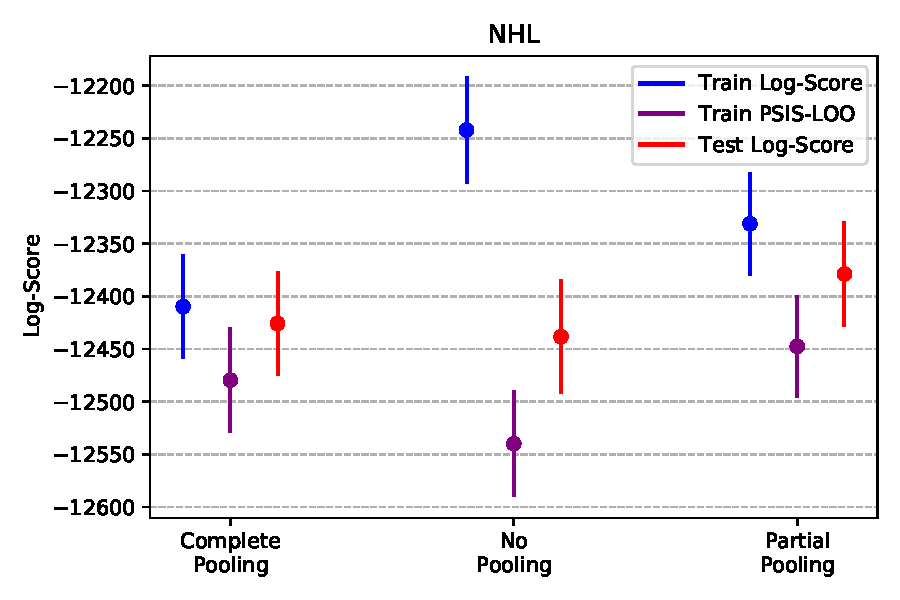
\includegraphics[width=0.5\textwidth]{figures/logscore_NHL.pdf}} 
	\subfloat[NBA]{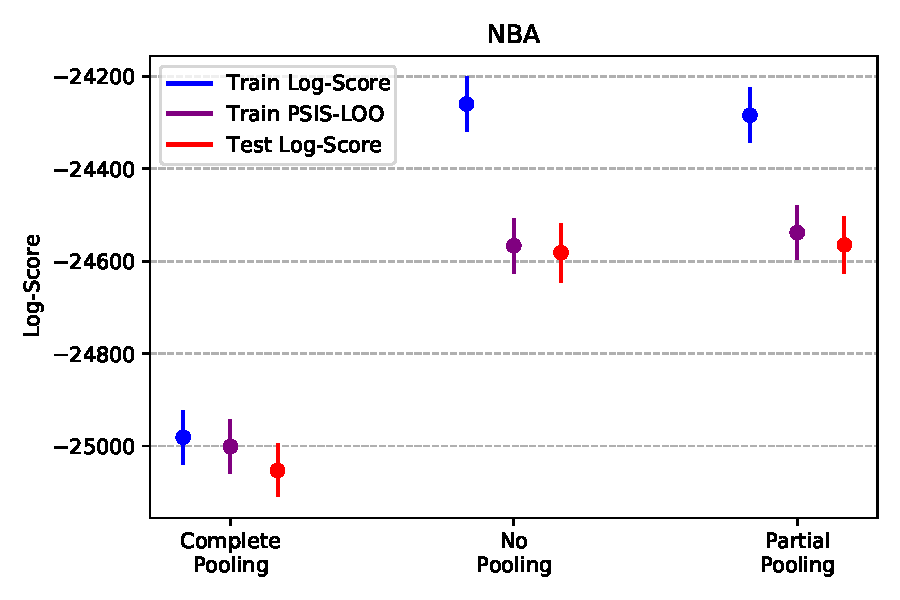
\includegraphics[width=0.5\textwidth]{figures/logscore_NBA.pdf}} \\
	\subfloat[MLB]{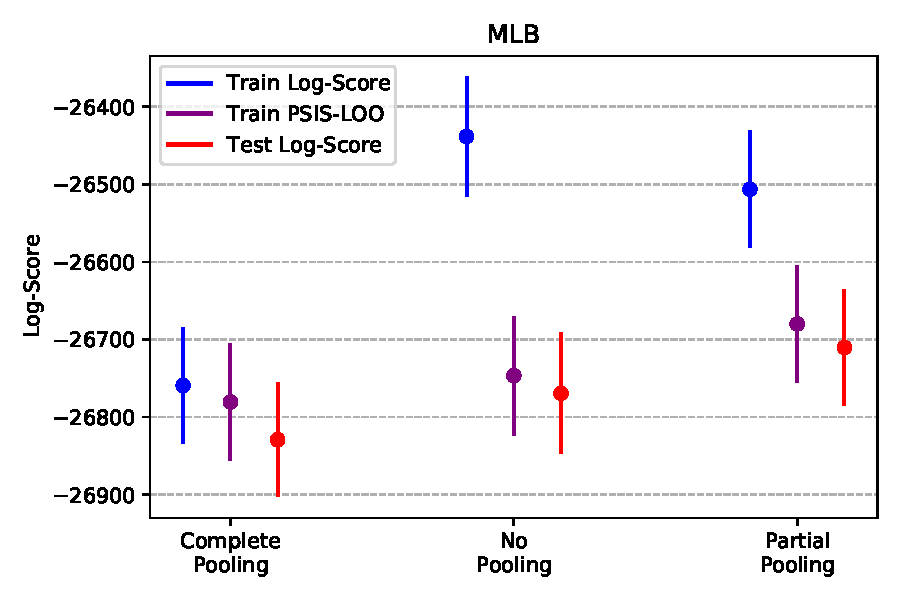
\includegraphics[width=0.5\textwidth]{figures/logscore_MLB.pdf}} 
	\subfloat[NFL]{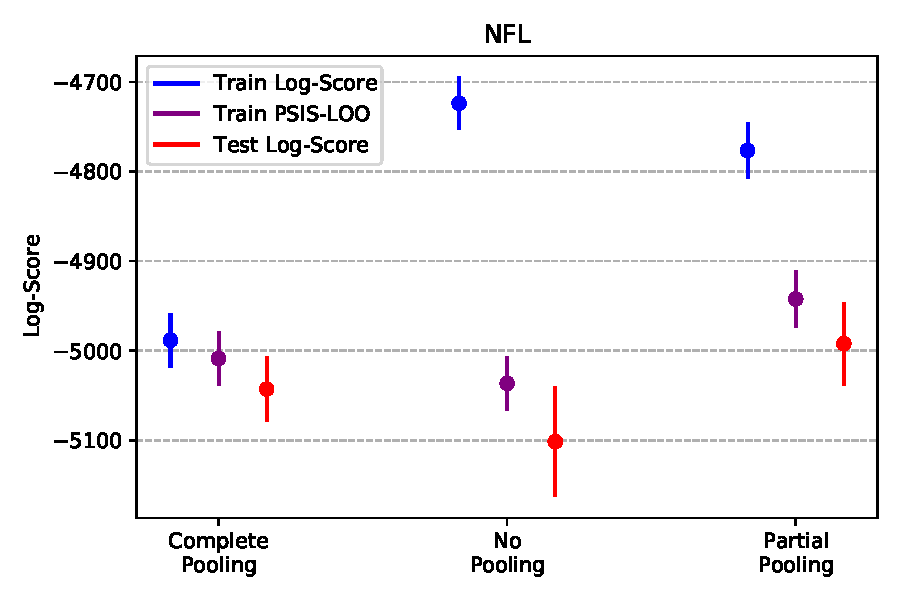
\includegraphics[width=0.5\textwidth]{figures/logscore_NFL.pdf}}
	\caption{Comparison of models via their Log-Score on train and test sets, as well as the PSIS-LOO estimated Log-Score, for each league. The complete-pooling model underfits, the no-pooling model overfits, and the partial-pooling model provides the best tradeoff in fitting the data while protecting against overfitting. The PSIS-LOO estimates consistently predict how the models would rank on an unseen test-set.}
	\label{fig:log_scores}
\end{figure}

\begin{figure}
	\subfloat[NHL]{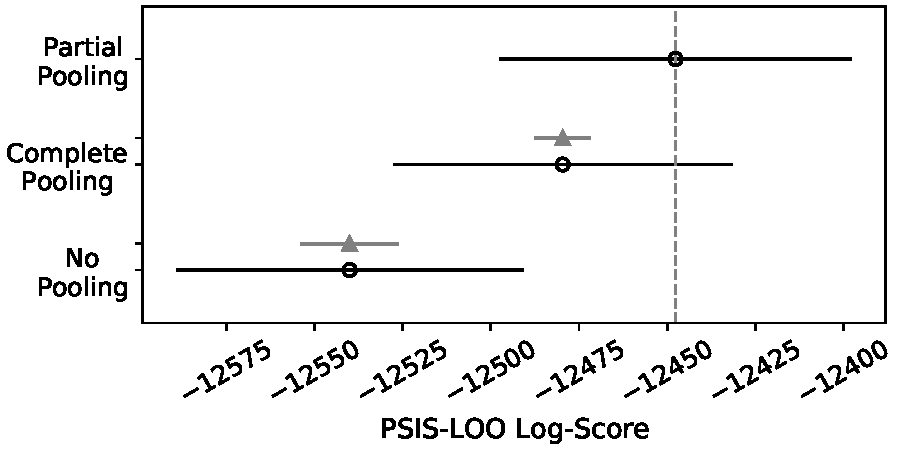
\includegraphics[width=0.5\textwidth]{figures/loo_nhl_no_title.pdf}} 
	\subfloat[NBA]{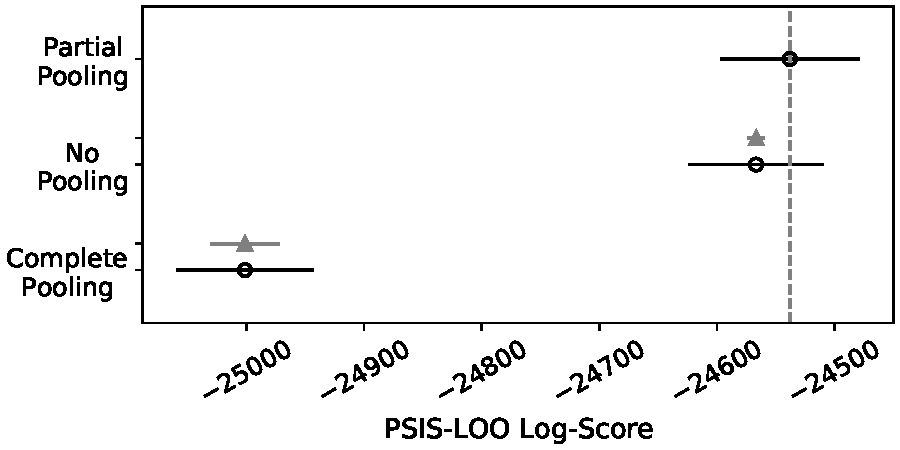
\includegraphics[width=0.5\textwidth]{figures/loo_nba_no_title.pdf}} \\
	\subfloat[MLB]{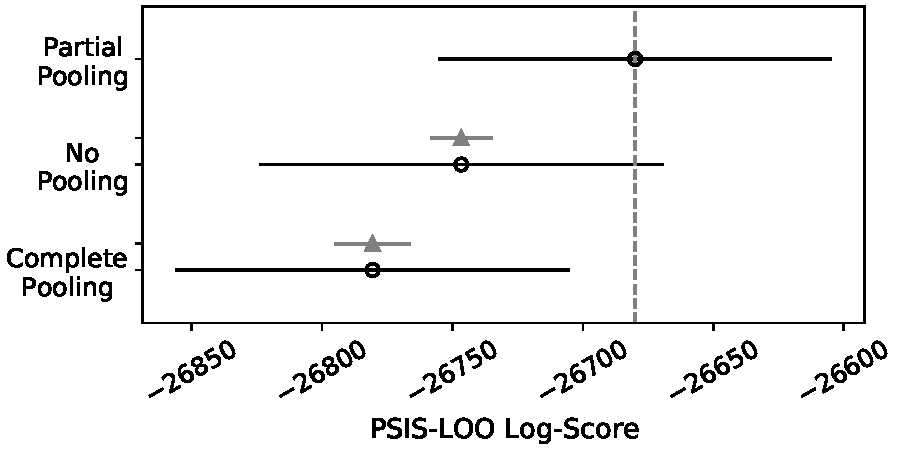
\includegraphics[width=0.5\textwidth]{figures/loo_mlb_no_title.pdf}} 
	\subfloat[NFL]{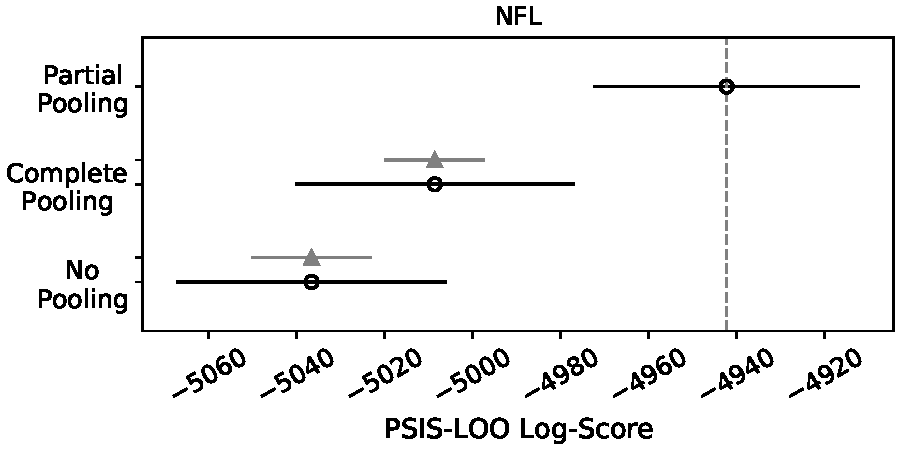
\includegraphics[width=0.5\textwidth]{figures/loo_nfl_no_title.pdf}}
	\caption{Comparison of models via their PSIS-LOO estimated Log-Score for each league, ranked from best (highest) to worst (lowest) on the y-axis. The black points and lines represent the point estimate and its standard error. The grey triangle and lines represent the estimated difference and the standard error of the difference for each model relative to the best model. The standard error of the difference is generally much smaller than the standard error of the estimate because errors in the estimates for each model are highly correlated.}
	\label{fig:psis_loo}
\end{figure}

The results of comparing models via their Log-Score, and how well PSIS-LOO is at estimating the out-of-sample performance, can be seen in Figure \ref{fig:log_scores}. The results show the same general trends across each league: 1) The complete-pooling model underfits the data compared to the other models, but it also overfits less compared to the other models as seen by its test-set performance not degrading as much, 2) The no-pooling model overfits the data the most as it generally has the best performance on the train-set but never has the best performance on the test-set, 3) The partial-pooling model consistently has the best train-set performance and is therefore the best performing model.

These results confirm the advantageous theory behind multilevel modelling explored in chapter ??. The multilevel model (partial-pooling model) consistently outperformed the complete-pooling model on both the train-set and the test-set. Interestingly the multilevel model consistently performed worse than the no-pooling model on the train-set but outperformed the no-pooling model on the test-sets. This is regularization at work and shows the efficacy of multilevel modelling over traditional regression. but fits the train-set worse than the no-pooling model.

The PSIS-LOO estimates of out-of-sample performance consistently ranked the models in the correct order measured by test-set performance, despite only having the train-set available to make these estimates. This shows how effective PSIS-LOO is at estimating out-of-sample performance, why it has become the current state of the art for model evaluation in Bayesian statistics, and why we opt for using PSIS-LOO estimates for ranking models in this thesis. We note that the exact magnitude of the PSIS-LOO estimates were sometimes over or under estimated relative to the test-set results, but that for a given dataset they were consistently over or under estimated. This is interesting because one of the additional contributions of Vehtari et el. (cite) was showing errors in PSIS-LOO estimates are highly correlated for the same dataset. Instead of more naive computations for the standard error, they instead derived an estimated for the standard error of the difference between models trained an evaluated on the same dataset. This new standard error generally provides tighter bounds that more accurately reflect the correlation in errors of PSIS-LOO estimates on the same dataset. A graphical representation of this can be seen in Figure \ref{fig:psis-loos}.

\begin{comment}
\begin{figure}
	\subfloat[NHL]{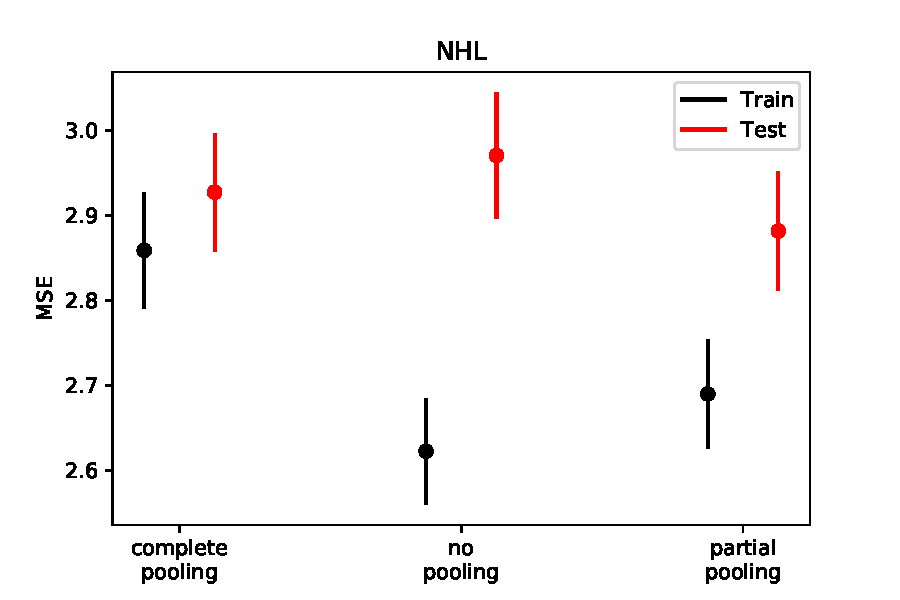
\includegraphics[width=0.5\textwidth]{figures/mse_nhl.pdf}} 
	\subfloat[NBA]{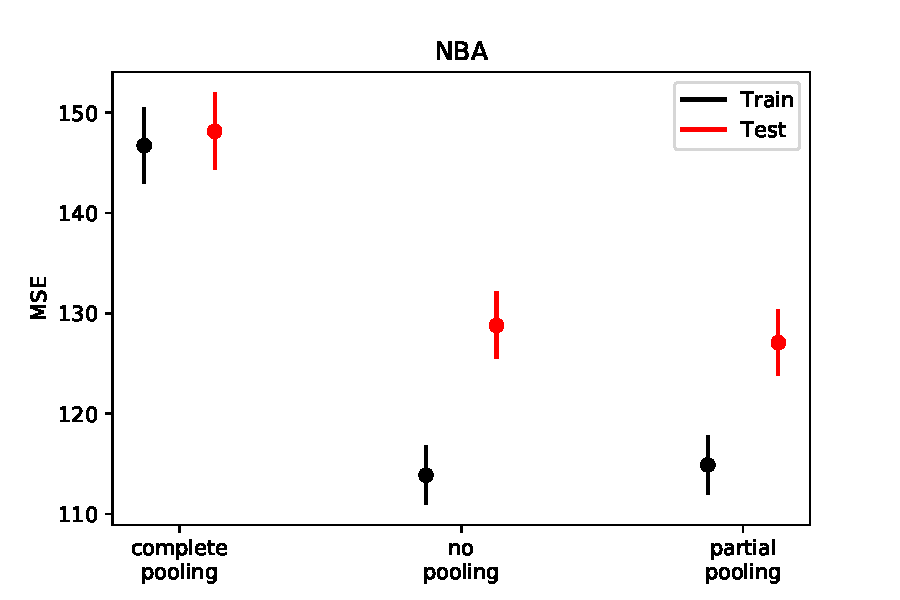
\includegraphics[width=0.5\textwidth]{figures/mse_nba.pdf}} \\
	\subfloat[MLB]{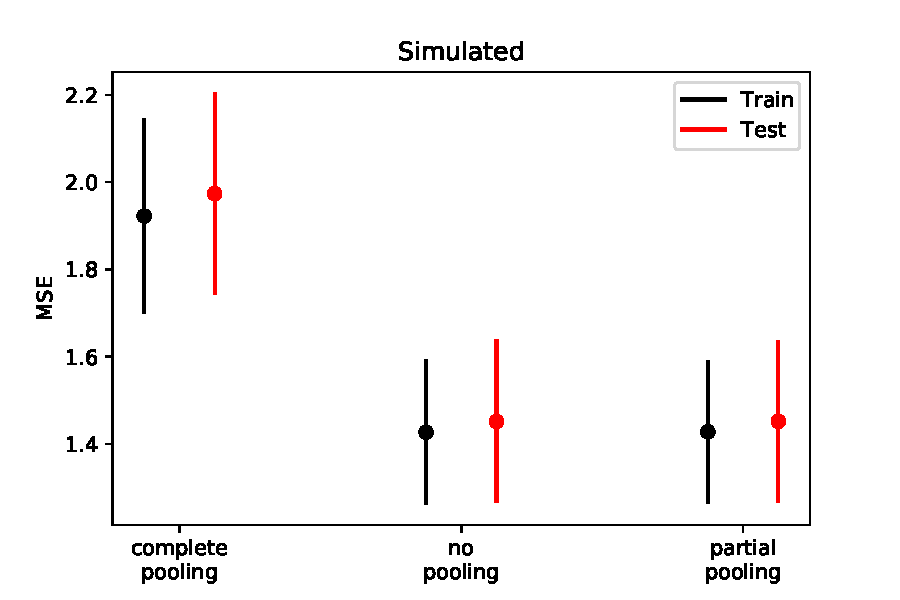
\includegraphics[width=0.5\textwidth]{figures/mse_mlb.pdf}} 
	\subfloat[NFL]{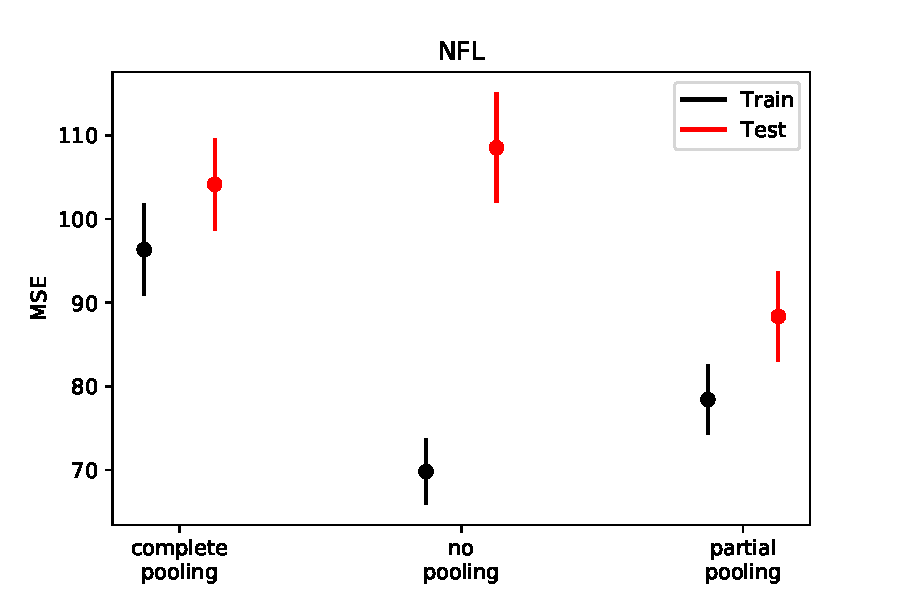
\includegraphics[width=0.5\textwidth]{figures/mse_nfl.pdf}}
	\caption{Comparison of models via their Mean-Squared-Error (MSE) on train and test sets for each league. The complete-pooling model underfits, the no-pooling model overfits, and the partial-pooling model provides the best tradeoff in fitting the data while protecting against overfitting.}
	\label{fig:mses}
\end{figure}

\begin{figure}
	\subfloat[NHL]{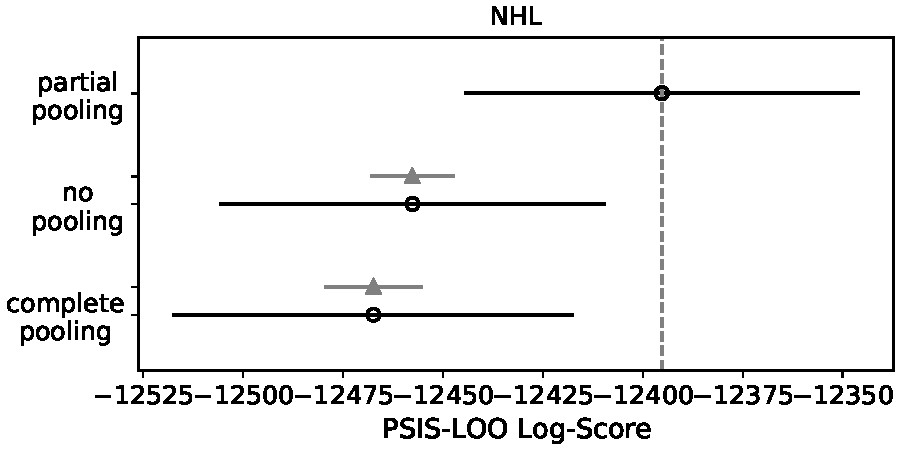
\includegraphics[width=0.5\textwidth]{figures/loo_nhl.pdf}} 
	\subfloat[NBA]{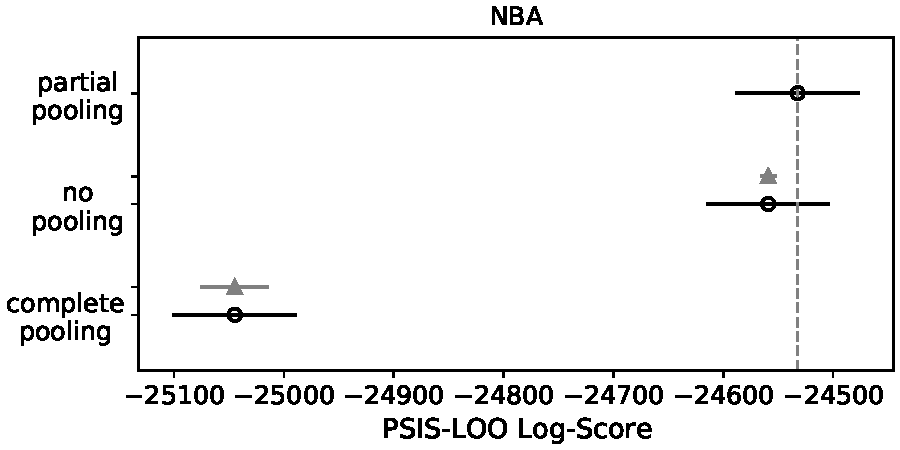
\includegraphics[width=0.5\textwidth]{figures/loo_nba.pdf}} \\
	\subfloat[MLB]{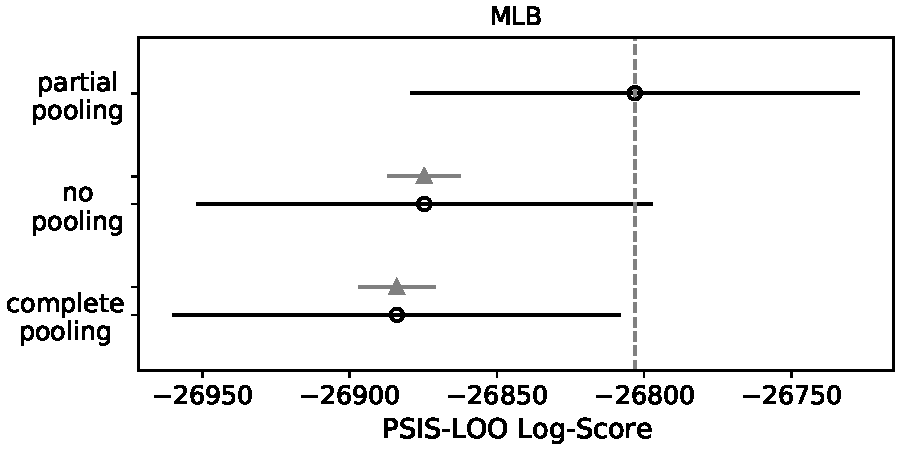
\includegraphics[width=0.5\textwidth]{figures/loo_mlb.pdf}} 
	\subfloat[NFL]{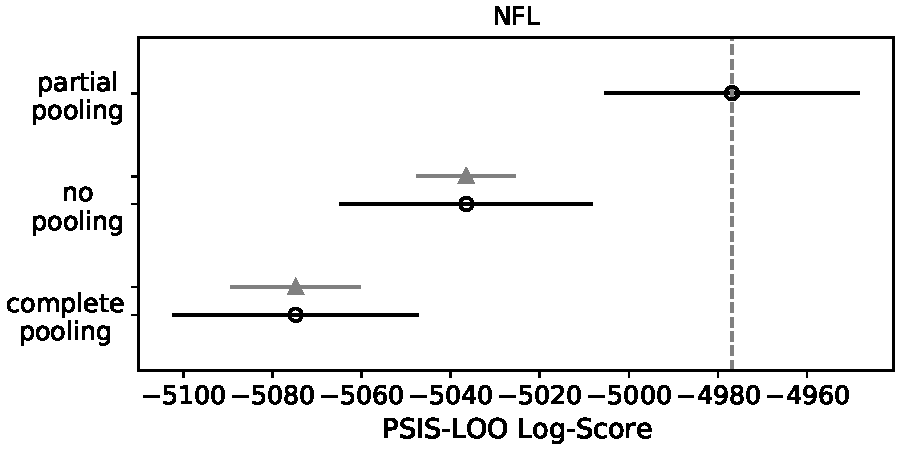
\includegraphics[width=0.5\textwidth]{figures/loo_nfl.pdf}}
	\caption{Comparison of models via their estimated out of sample performance as measured by PSIS-LOO. Since the estimates are computed in the same way on the same data, their errors are highly correlated and the grey error bars represent a more accurate estimate of the standard error of the estimates relative to the best performing model.}
	\label{fig:psis-loos}
\end{figure}
\end{comment}

\subsection{Negative Binomial Regression}

\begin{figure}
	\centering
	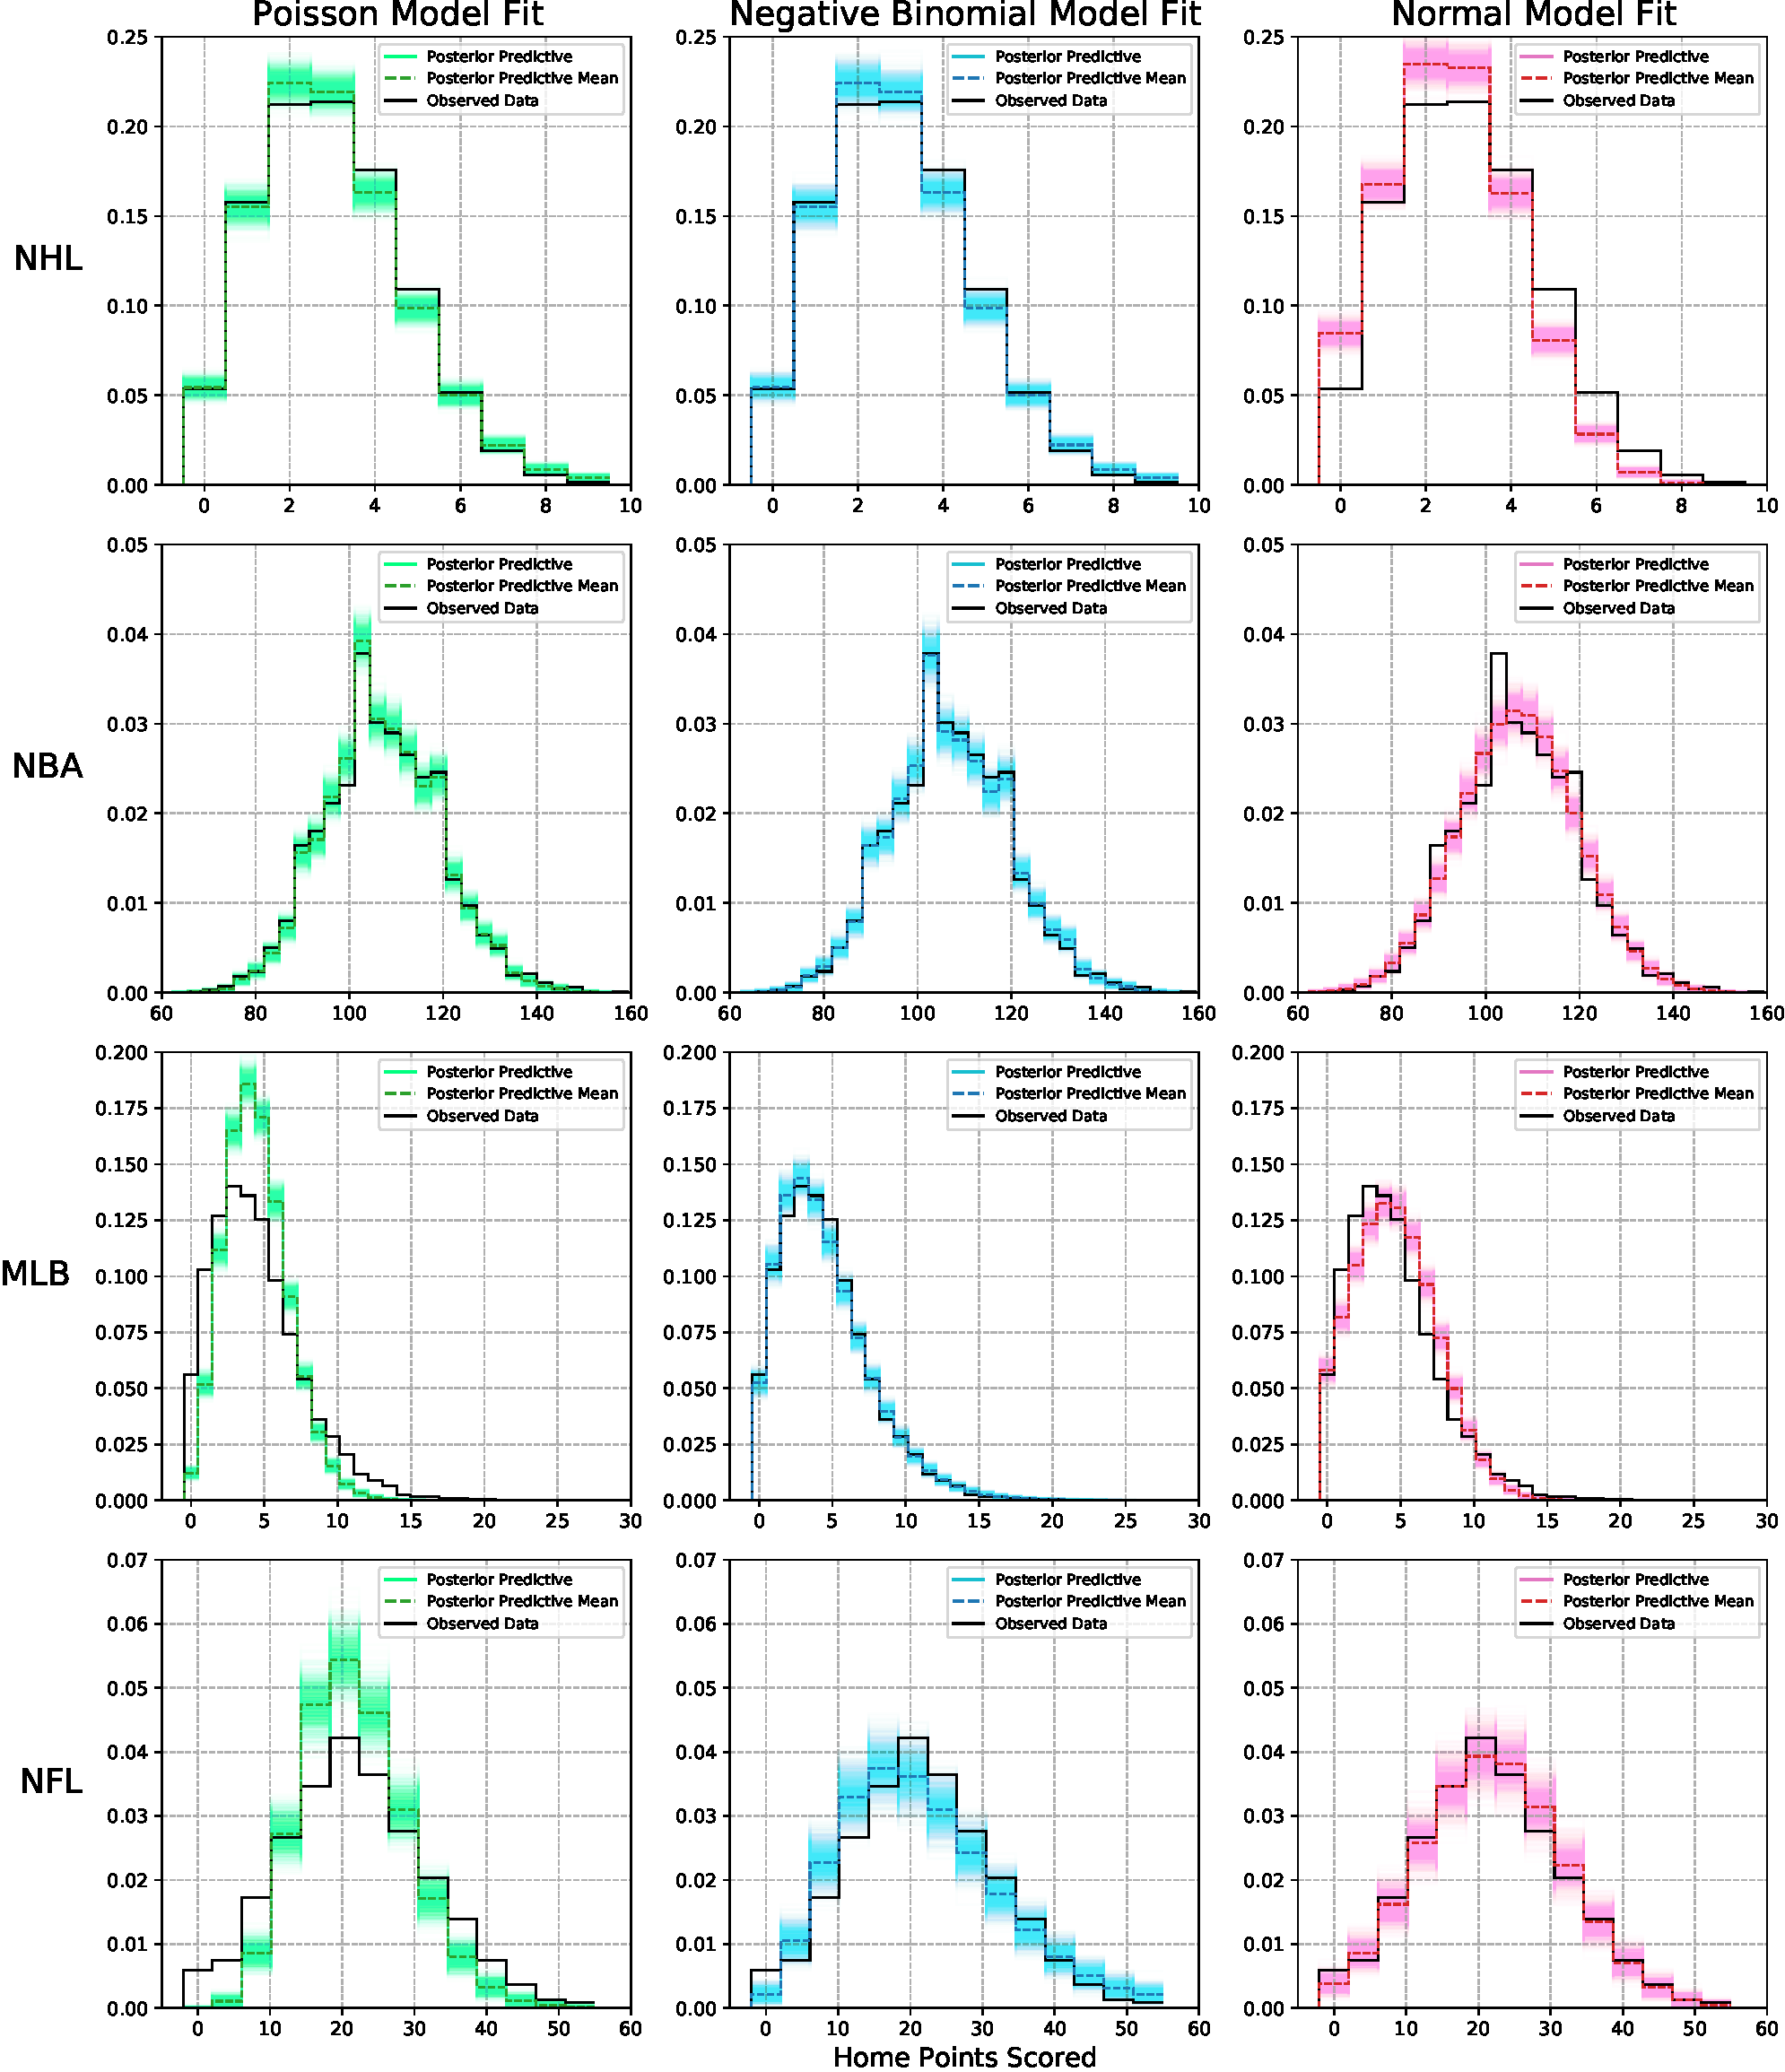
\includegraphics[width=\textwidth]{figures/Figure_3.pdf}
	\caption{Comparison of distribution of home points in the models and the observed data for each league. The Negative Binomial model noticeably provides a better overall fit across each league.}
	\label{fig:comparisons}
\end{figure}

The differences in model fit for the various likelihood distributions considered can be seen visually in Figure \ref{fig:comparisons}. Visually inspecting the distributions in Figure \ref{fig:comparisons} is known as a Posterior Predictive Check (PPC) as described in section ??. The PPCs in Figure \ref{fig:comparisons} are performed by plotting the distribution of observed home point totals in black along with 2000 sampled model fits in green for Poisson, blue for Negative Binomial, and red for Normal; with the respective mean model fits across the 2000 samples as dashed lines. The differences between the Poisson and Negative Binomial models becomes increasingly apparent for the leagues with greater overdispersion, while the Normal model comparatively struggles for each league except the NFL where both the Normal and Negative Binomial greatly outperform the Poisson model. Because the point totals of the sports we are considering are positive integers prone to overdispersion and based on the results in Table \ref{tab:loo} and Figure \ref{fig:comparisons}, we conclude that the Negative Binomial distribution is the most appropriate for regression modelling professional hockey, basketball, baseball, and American football.

\begin{table}
\centering
\begin{tabular}{c@{\hskip0.35in}c@{\hskip0.35in}c@{\hskip 0.25in}c@{\hskip 0.25in}c@{\hskip 0.15in}c}
\toprule
& \boldmath$\sigma_p$ & \textbf{Model} & \textbf{PSIS-LOO} & \textbf{dLOO} & \textbf{dSE}\\
\midrule
&& \textbf{Poisson} & \textbf{-24761.3} & - & -\\
NHL & 0.99 & NB & -24761.5 & 0.2 & 0.2\\
&& Normal & -25140.9 & 379.5 & 23.4\\
\midrule
&& Poisson & -49018.3 & 53.5 & 11.0\\
NBA & 1.50 & \textbf{NB} & \textbf{-48964.8} & - & -\\
&& Normal & -48981.9 & 16.6 & 7.5\\
\midrule
&& Poisson & -57458.7 & 4115.8 & 120.9\\
MLB & 2.27 & \textbf{NB} & \textbf{-53342.9} & - & -\\
&& Normal & -55696.8 & 2353.17 & 65.1\\
\midrule
&& Poisson & -11751.2 & 2042.5 & 119.0\\
NFL & 4.56 & NB & -9841.7 & 133.0 & 22.1\\
&& \textbf{Normal} & \textbf{-9708.7} & - & -\\
\bottomrule
\end{tabular}
\caption{Comparison of estimated negative log-likelihood of leave-one-out cross-validation (LOO) for each model across each league. The differences between the Poisson, Negative Binomial (NB), and Normal models are reported relative to the best fitting model (dLOO) for each league; along with the standard error of the estimated differences (dSE). The dispersion statistic, \(\sigma_p\), indicates how much greater the variance is than the mean for point totals in each league and signals overdispersion when \(\sigma_p > 2\). The NB model noticeably outperforms the Poisson model for leagues with greater overdispersion (MLB and NFL) while being nearly identical for leagues with little to no overdispersion (NHL and NBA). The NB model also outperforms the Normal model in each league except the NFL where they are close to one another while both vastly outperforming the Poisson model.}\label{tab:loo}
\end{table}

\subsection{Inferring Home Advantage}

- similar to paper

\begin{figure}
	\centering
	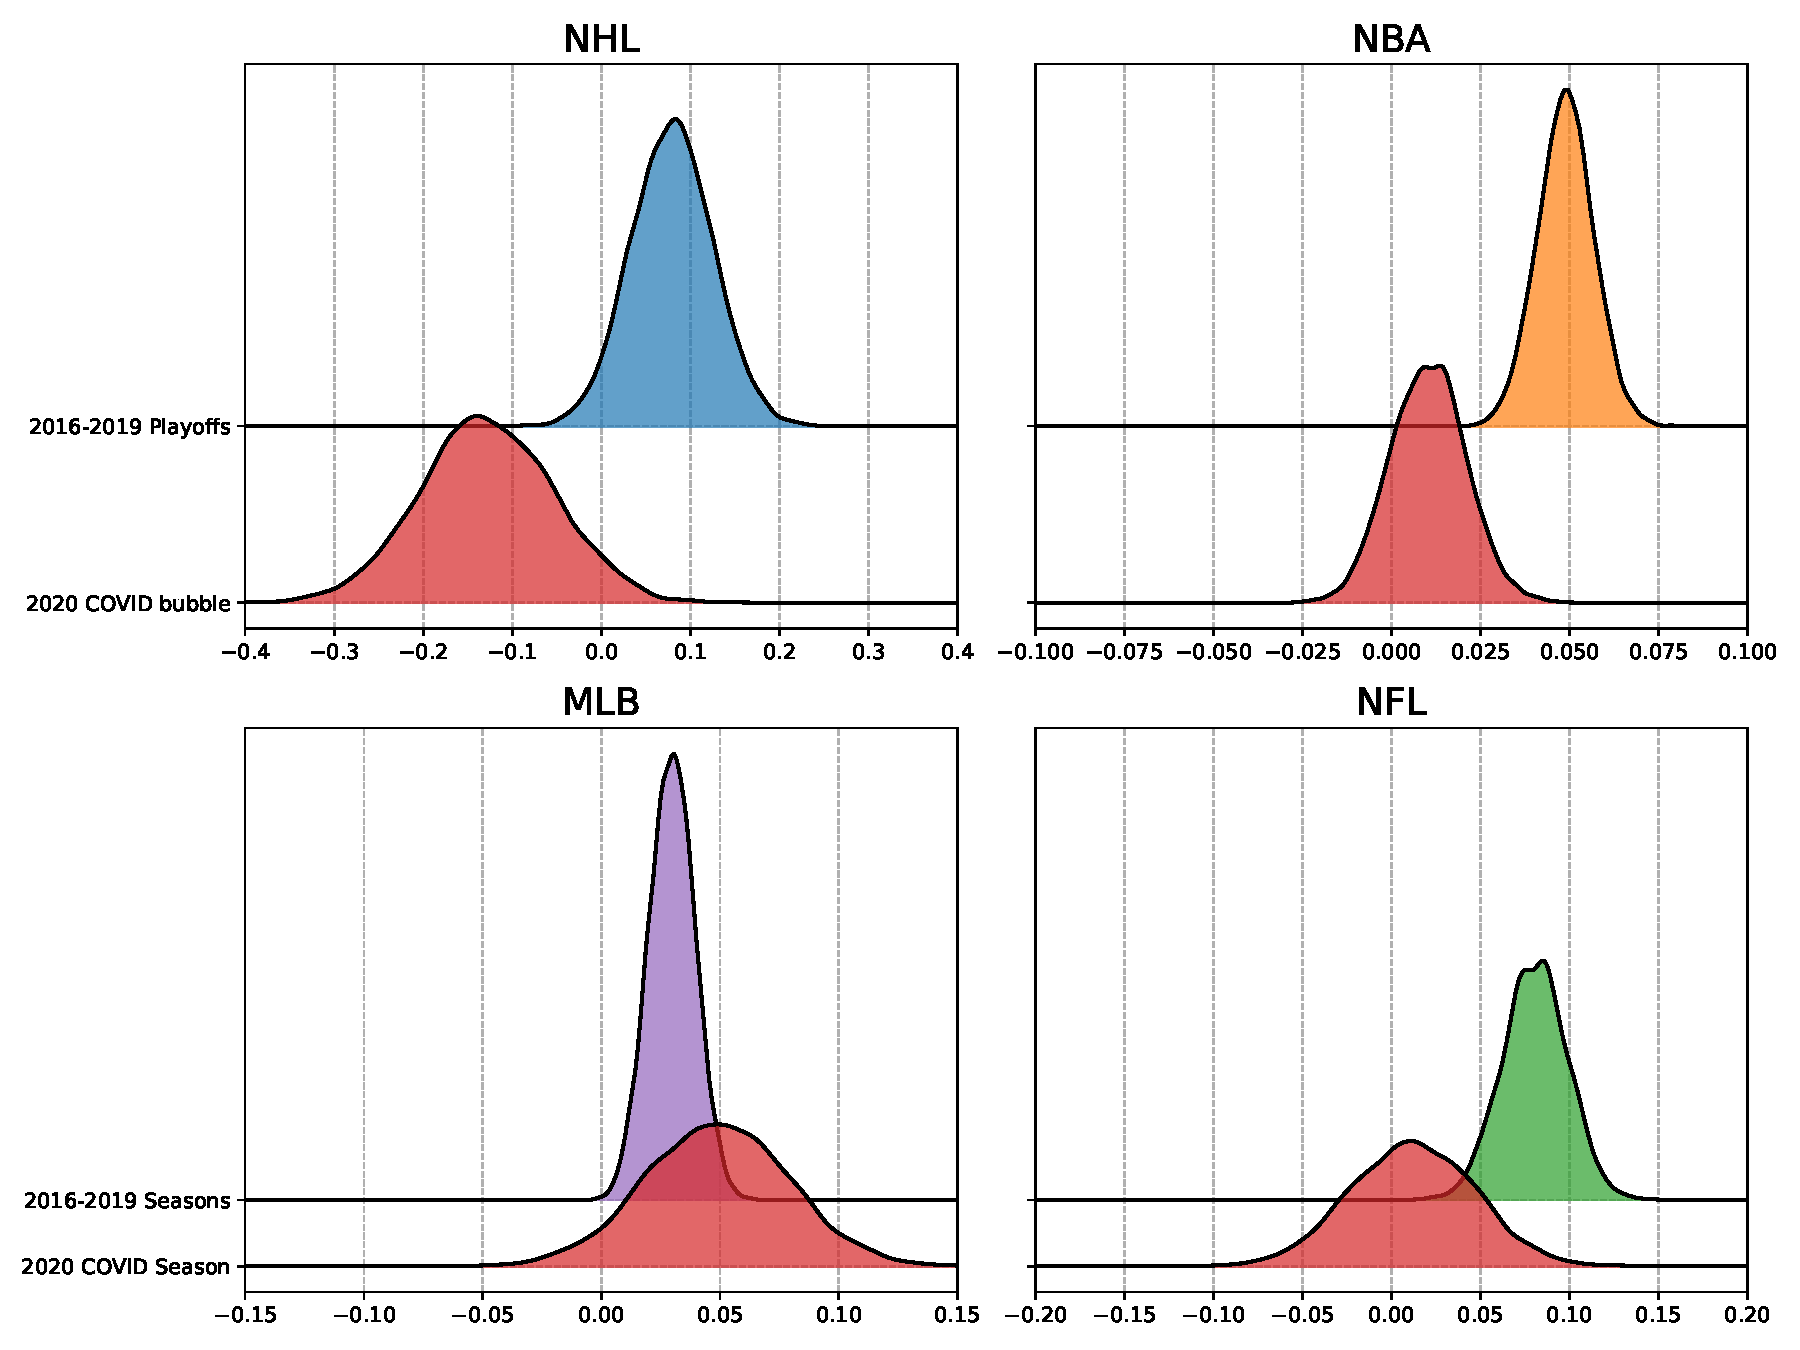
\includegraphics[width=0.9\textwidth]{figures/Figure_1.pdf}
	\caption{Distributions of the estimated home advantage for the NHL, NBA, MLB, and NFL for pre and post COVID adjusted seasons. Home advantage for playoffs are reported for NHL and NBA because that is when their COVID restricted games took place. Home advantage for regular season is reported for MLB and NFL as their respective playoff seasons are too small for stable results. Red distributions represent COVID-19 bubble adjusted seasons.}
	\label{fig:ha_pooled}
\end{figure}

The distributions for the estimates of the home advantage parameters from pooling the previous four pre-COVID-19 seasons/playoffs together can be seen in Figure \mbox{\ref{fig:ha_pooled}} with the COVID-19 restricted season/playoffs coloured red. The peaks of these distributions represent the most likely values for the home advantage parameter and their width represents the uncertainty in these estimates. We can use these distributions to directly measure the probability the home advantage parameter is less than the previous seasons. The leftward shift of the distribution for the COVID-19 restricted season/playoffs suggests that home advantage decreased in the NHL, NBA, and NFL while not changing for the MLB.

Figure \mbox{\ref{fig:ha_main}} shows results from estimating home advantage individually for each prior season. This more granular view of pre-COVID-19 home advantage reveals greater season-to-season variation in home advantage that is missing in Figure \mbox{\ref{fig:ha_pooled}}. Nevertheless, the year-over-year estimates in Figure \mbox{\ref{fig:ha_main}} show the results of reduced home advantage in COVID-19 restricted season/playoffs holding for the NHL, NFL, and NBA, albeit with a single past season with lower home advantage in both the NFL and NBA. The remainder of this section examines these estimated distributions and their implications.

For the NHL and NBA data, Figures \mbox{\ref{fig:ha_pooled}} and \mbox{\ref{fig:ha_main}} and our analysis focus on their playoff seasons because the NHL and NBA COVID-19 seasons only took place during their playoff seasons. In contrast, the MLB and NFL had COVID-19 restrictions for their entire seasons, therefore, Figures \mbox{\ref{fig:ha_pooled}} and \mbox{\ref{fig:ha_main}}, and our analysis for those leagues are focused on their regular season games. Focusing on the MLB and NFL regular seasons is not only convenient but arguably necessary as their playoff seasons consist of much fewer games than the NHL and NBA playoff seasons, resulting in high uncertainty of parameter estimates. The NHL and NBA regular season results as well as the MLB and NFL playoff results are provided in the supplementary materials.

The home advantage parameter, $\beta$, represents a multiplier of $\text{exp}(\beta)$ applied to expected points. For example, an estimated home advantage parameter for the NBA of $0.05$ represents a $\text{exp}(0.05) \approx 1.0513$ multiplier on expected points or an increase in expected points of 5\%. With average points scored in the NBA being around 107 this would translate to approximately a 5-point home advantage on average in the NBA playoffs. We provide a full description and interpretation of the model in the Methods section.

For the NHL data, the results in both Figures \mbox{\ref{fig:ha_pooled}} and \mbox{\ref{fig:ha_main}} show the home advantage parameter confidently above 0 for pre-COVID-19 seasons and confidently below 0 for the COVID-19 bubble. The probability the home advantage parameter $(\beta)$ is less than 0 for the COVID-19 bubble is $\Pr(\beta < 0) = 0.95$. The probability the home advantage parameter is less than the previous playoff seasons mean of $0.081$ is $0.998$. These results give strong evidence that home advantage in the NHL was negatively impacted by the COVID-19 bubble.

For the NBA data, the pooled home advantage parameter estimate in Figure \mbox{\ref{fig:ha_pooled}} is confidently above 0 and tightly around 0.05. For the COVID-19 affected playoffs, the probability the home advantage is less than 0 is only $0.17$, but the probability that it is less than the pre-COVID-19 mean of 0.05 is $0.999$, suggesting that home advantage in the NBA was negatively impacted by the COVID-19 bubble. However, when examining the year-to-year estimates of prior seasons in Figure \mbox{\ref{fig:ha_main}} we see a decreasing trend in home advantage in the NBA playoffs with the estimate for the NBA playoffs in 2017 appearing as almost as much of an outlier as the COVID-19 estimate. This suggests the decreased home advantage in the COVID-19 could potentially be a random outlier. The uncertainty in these estimates means we can not make definitive conclusions in the absence of more data. We conclude that it is probable that home advantage in the NBA decreased in the COVID-19 bubble but not as definitively as the NHL results.

For the MLB data, the home advantage parameter is surprisingly likely to be slightly greater than it had been in previous seasons. The probability the home advantage parameter is less than the mean of the previous seasons is $\Pr(\beta < 0.036) = 0.26$. When comparing the COVID-19 estimate to the previous seasons in Figure \mbox{\ref{fig:ha_main}} there appears to be no noteworthy difference. This gives evidence that home advantage in the MLB was unlikely to be negatively impacted by the COVID-19 restrictions and was likely unaffected by the restrictions.

For the NFL data, the pooled home advantage parameter estimate in Figure \mbox{\ref{fig:ha_pooled}} is confidently above 0 with a mean of 0.078. For the COVID-19 affected season, the probability the home advantage is less than 0 is $0.388$, but the probability that it is less than the pre-COVID-19 mean of 0.078 is $0.976$, suggesting that home advantage in the NFL was negatively impacted by the COVID-19 restrictions. However, when examining the year-to-year estimates of prior seasons there is a clear pattern of home advantage decreasing in the NFL and even being lower in 2019 than it was in the 2020 COVID-19 adjusted season. We argue the results in Figure \mbox{\ref{fig:ha_main}} are enough to overturn the results in Figure \mbox{\ref{fig:ha_pooled}} and conclude that home advantage in the NFL was not impacted from its previous trend by the COVID-19 restrictions.

In summary, results for pooled (Figure~\mbox{\ref{fig:ha_pooled}}) and individual~(Figure~\mbox{\ref{fig:ha_main}}) past seasons give strong evidence that home advantage in the NHL was negatively impacted during the COVID-19 restricted playoff season and that home advantage in the MLB was unaffected by the restrictions. Pooled past season results also suggest home advantage was negatively impacted by the COVID-19 restricted seasons for the NBA and NFL, however a closer examination of the individual past season results reveals a trend of decreasing home advantage over the past few seasons, which may partly account for the lower home advantage found during NBA and NFL COVID-19 restrictions.

\begin{figure}
	\centering
	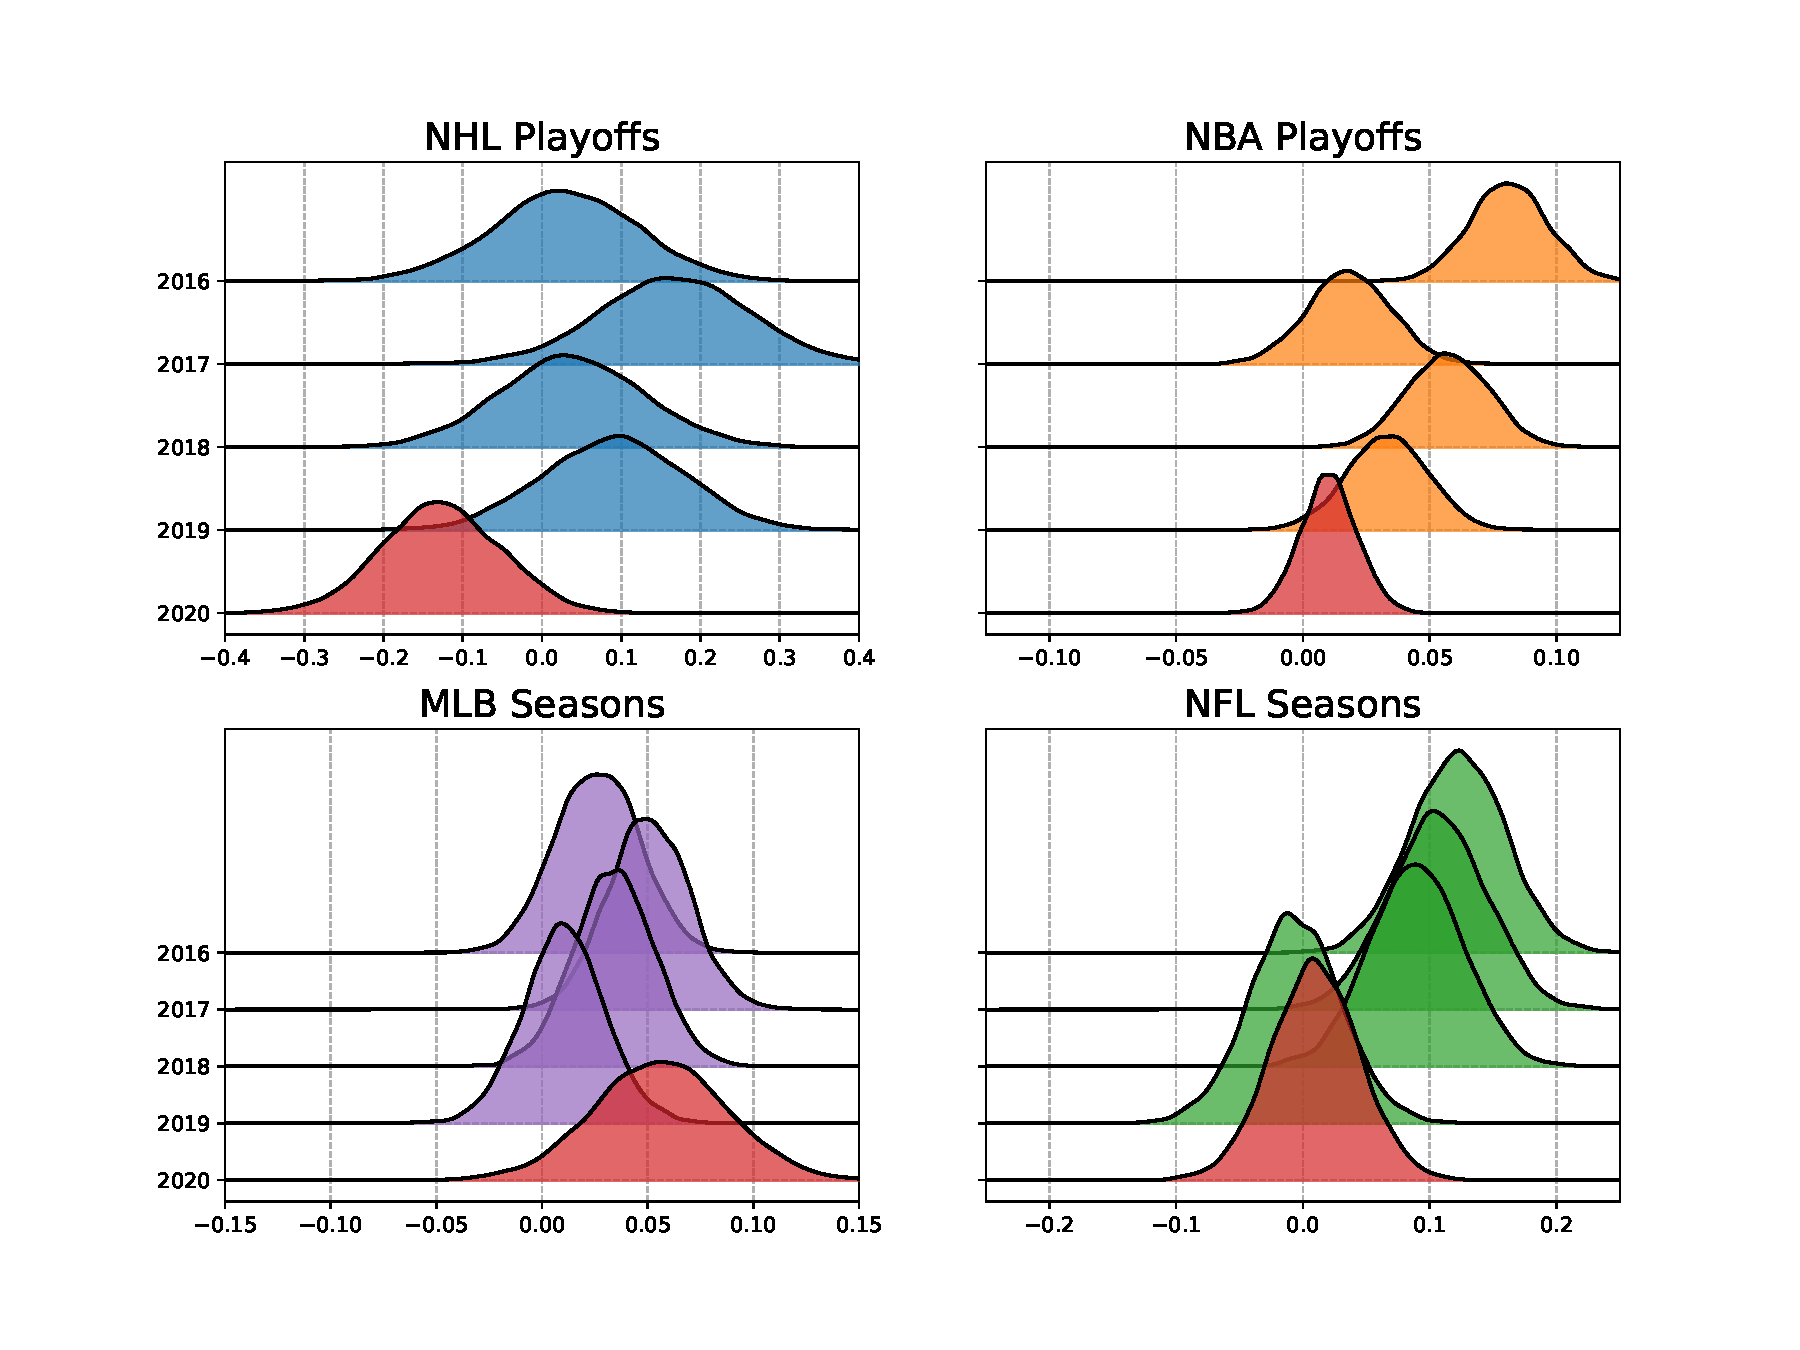
\includegraphics[width=\textwidth]{figures/Figure_2.pdf}
	\caption{Distributions of the estimated home advantage for the NHL, NBA, MLB, and NFL over the past 5 seasons from 2016-2020. Home advantage for playoffs are reported for NHL and NBA because that is when their COVID restricted games took place. Home advantage for regular season is reported for MLB and NFL as their respective playoff seasons are too small for stable results. Red distributions represent COVID-19 bubble adjusted seasons.}
	\label{fig:ha_main}
\end{figure}

\chapter{Conclusions}
The results of our model when pooling the previous seasons prior to COVID-19 (Figure \mbox{\ref{fig:ha_pooled}}) show a noticeable decrease in home advantage for the NHL, NBA, and NFL with no noticeable change in home advantage for the MLB. However, while the year-over-year estimates (Figure \mbox{\ref{fig:ha_pooled}}) corroborate these findings to be significant for the NHL and MLB, they show the results are potentially weaker for the NBA and NFL. We argue that the results in Figure \mbox{\ref{fig:ha_main}} reveal that home advantage in the NFL was already decreasing leading up to the 2020 season and that the 2020 COVID-19 restricted season had no significant impact on home advantage in the NFL. We further argue that the NBA COVID-19 restricted season may potentially be an outlier similar to the 2017 playoffs. This means we can not be as confident in our conclusions about home advantage decreasing in the NBA as we are with the NHL. We argue the results give evidence that it is likely home advantage decreased in the NBA but we can not be certain with the limited sample we have.

%The results of our model shows strong evidence of home advantage being a real positive phenomenon in the NHL and NBA prior to the COVID-19 bubble seasons and that the COVID-19 bubble negatively impacted home advantage by removing it almost entirely (Figure \ref{fig:ha_results} (a) and (b)). In contrast, the MLB and NFL showed a trend of relatively smaller home advantage parameter estimates in recent years and showed little to no evidence of COVID-19 restrictions having an impact on home advantage in these sports (Figure \ref{fig:ha_results} (c) and (d)).

If we contrast the COVID-19 restrictions in the NHL and NBA to the MLB and NFL, there are two notable differences. First, the NHL and NBA had much stricter COVID-19 bubbles where teams did not travel to each others stadiums, whereas the MLB and NFL did travel to the various stadiums and only restricted fans attending. This suggests that the lack of travel and home city familiarity contributes to home advantage more than a home crowd effect, and therefore results in a greater drop in home advantage in the leagues that had a strict bubble compared to the leagues that allowed travel and play at home stadiums. This agrees with McHill \& Chinoy \cite{McHill2020} and gives further evidence to the cause of home advantage being more attributable to the general effect of travel. The second difference is the relatively small to no home advantage that the model infers for the MLB and NFL relative to the strongly positive home advantage in recent years found in the NHL and NBA. While we can not fully tease out which of these two differences is stronger, this opens up potential for future work as these leagues continue to play through the COVID-19 pandemic. It will be interesting to see if home advantage returns in the NHL and NBA as they shift toward fewer restrictions similar to the MLB and NFL.

The strongest result for a decrease in home advantage due to COVID-19 restrictions was seen in the NHL. We note that this is particularly interesting because the NHL is somewhat unique to the other leagues, because the home team has an extra difference; they get the last change during stoppages of play, meaning they get to decide player matchups. An analysis of this effect has been carried out by Meghan Hall \cite{Hall2020} who concluded that home teams benefit when they get to control matchups and argued that this benefit should not be discounted during the 2020 COVID-19 bubble season. The results of our model, however, seem to indicate that no home advantage existed during the NHL's COVID-19 bubble and suggests the effect of last change in the NHL is potentially not as impactful as previously thought.

We have also shown how using the Negative Binomial distribution as the likelihood function for our regression model outperforms the Poisson distribution for sports with overdispersion in their point totals such as the MLB and NFL, while still performing just as well as the Poisson distribution when there is little to no overdispersion such as in the NHL and NBA. We showed the Negative Binomial distribution also outperforms the Normal distribution across all leagues except for the NFL where both models vastly outperformed the Poisson distribution. We argue this is because the Negative Binomial distribution effectively represents positive integers like the Poisson distribution while having an extra parameter, like the Normal distribution, to account for overdispersion which represents a greater spread in the data due to greater variance.

We have further shown that a multilevel regression model outperforms traditional regression and simple averaging as measured by out-of-sample predictive fit. Our experiments showed that simple averaging (complete-pooling of, or ignoring, relative team strengths) underfits the data, and that traditional regression is poised to overfit the data. Our multilevel model provides the best tradeoff in providing a better fit to the datasets while preventing overfitting. Combined with Negative Binomial regression, we have introduced a multilevel regression model that fits the data better than previous works and therefore gives better opportunity to infer home advantage.

Our Bayesian regression model has three key advantages over traditional methods for inferring home advantage. First, methods that rely on correlations among raw statistics fail to account for factors such as relative team strengths. For example, a weaker team may have a poor home win percentage because they have a poor overall win percentage. That same team; however, may perform better at home than they do at other stadiums whilst still losing to stronger opponents and vice versa. This discrepancy can be further impacted by imbalanced schedules where teams do not face the same opponents as each other in a perfectly balanced manner. While some studies recognize this discrepancy, they often claim that it is a small effect that can be ignored \cite{Pollard2005a} without showing evidence. We argue that while these claims may hold up for analyses spanning decades they are not appropriate for the short COVID-19 restricted seasons we are considering. Furthermore, these issues and any debate over how much of an effect they have is most reliably mitigated by adjusting for varying team strengths when trying to infer home advantage. Regression analysis methods are primarily used for their ability to account for multiple factors when performing inference, and as such they are most appropriate for our focus of analyzing home advantage. Second, the Bayesian framework gives more interpretable results and more flexibility in model building than classical regression methods. This can be seen in the results of the Bayesian framework being distributions for the estimates of each parameter in our model. In this way the implied probability and corresponding uncertainty of parameter estimates are still rigorously defined while being directly measurable and more intuitive to understand than traditional Frequentist methods of confidence intervals and p-values. Third, with advancements in computational Bayesian statistics, such as Probabilistic Programming languages \cite{pymc3} and Hamiltonian Monte Carlo (HMC) \cite{Betancourt2017}, we are able to easily define and compute flexible and complex models using various likelihood functions with ease instead of being limited to traditional methods like Normal and Poisson regressions more traditionally used in sports modelling \cite{Lopez2018} \cite{Glickman1998} \cite{Karlis2003} \cite{Baio2010} \cite{Benz2020}.

While our model has produced some interesting results, it is worth discussing some of its limitations and areas for future work and improvement. The most notable limitation is that the COVID-19 lockout and restricted seasons are unprecedented and come with additional caveats such as protocols for testing, impact of positive tests, reduced practices, and players being away from their families, that extrapolating all results to home advantage or fan impact alone does not address all the possible factors influencing player and team performance. The model also does not account for travel or rest before games as a potential confounding factor for home advantage. This was ignored primarily due to it being irrelevant for the NHL and NBA COVID-19 bubbles, but for the less restrictive MLB and NFL seasons as well as future COVID-19 restricted seasons this could be a potential factor worth exploring. The model could benefit by including group level factors when estimating the offensive and defensive strengths of teams. The multilevel structure of the Bayesian framework we have adopted naturally allows for such inclusions \cite{Gelman2006} \cite{Gelman2014} \cite{McElreath2020}. For example, we hypothesize that advanced analytics metrics such as expected goals (xG) and corsi in hockey, regularized adjust plus-minus (RAPM) in basketball, hitter splits and park factors in baseball, yards gained/allowed above/below expected in football, could all be leveraged to improve team strength estimates. This could also include personnel differences such as the effect of star players being injured, back-up goalies starting, or starting pitchers being included in the estimates of a teams relative strength for a given game. These inclusions are beyond the scope of this work as these analytics and personnel changes and their effect differ greatly across different sports. In future work, we hope to focus on an individual sport and include such factors, using the current model as a baseline to compare against. Our model is also limited by focusing on only point totals to infer home advantage, while some previous works also analyze differences in penalties to assess a home advantage in the officiating of games \cite{Benz2020} \cite{Unkelbach2010} \cite{Buraimo2010} \cite{Dohmen2016}. This was excluded from this work because of how much penalties and their effect differ across the various sports we considered, but is something we hope to explore in the future when analyzing a single sport in more depth.


%%%%%%%%%%%%%%%%%%%%%%%%%%%%%%%%%%%%%%%%%%%%%%%%%%%%%%%%%%%%%%%%
% The Bibliograpy should go here. BEFORE appendices!
%%%%%%%%%%%%%%%%%%%%%%%%%%%%%%%%%%%%%%%%%%%%%%%%%%%%%%%%%%%%%%%%


% Typeset the Bibliography.  The bibliography style used is "plain".
% Optionally, you can specify the bibliography style to use:
% \uofsbibliography[stylename]{yourbibfile}

\uofsbibliography{880Paper}

% If you are not using bibtex, comment the line above and uncomment
% the line below.  
%Follow the line below with a thebibliography environmentand bibitems.  
% Note: use of bibtex is usually the preferred method.

%\uofsbibliographynobibtex


%%%%%%%%%%%%%%%%%%%%%%%%%%%%%%%%%%%%%%%%%%%%%%%%%%%%%%%%%%%%%%%%%%%%%%%%%
% APPENDICES
%
% Any chapters appearing after the \appendix command get numbered with
% capital letters starting with appendix 'A'.
% New chapters from here on will be called 'Appendix A', 'Appendix B'
% as opposed to 'Chapter 1', 'Chapter 2', etc.
%%%%%%%%%%%%%%%%%%%%%%%%%%%%%%%%%%%%%%%%%%%%%%%%%%%%%%%%%%%%%%%%%%%%%%%%%%

% Activate thesis appendix mode.
\uofsappendix

% Put appendix chapters in the appendices environment so that they appear correcty
% in the table of contents.  You can use \input's here as well.
\begin{appendices}

\chapter{Sample Appendix}

Stuff for this appendix goes here.

\chapter{Another Sample Appendix}

Stuff for this appendix goes here.

\end{appendices}

\end{document}
